% -*- latex -*-
%%%%%%%%%%%%%%%%%%%%%%%%%%%%%%%%%%%%%%%%%%%%%%%%%%%%%%%%%%%%%%%%
%%%%%%%%%%%%%%%%%%%%%%%%%%%%%%%%%%%%%%%%%%%%%%%%%%%%%%%%%%%%%%%%
%%%%
%%%% This text file is part of the source of 
%%%% `Introduction to High-Performance Scientific Computing'
%%%% by Victor Eijkhout, copyright 2012
%%%%
%%%% This book is distributed under a Creative Commons Attribution 3.0
%%%% Unported (CC BY 3.0) license and made possible by funding from
%%%% The Saylor Foundation \url{http://www.saylor.org}.
%%%%
%%%%
%%%%%%%%%%%%%%%%%%%%%%%%%%%%%%%%%%%%%%%%%%%%%%%%%%%%%%%%%%%%%%%%
%%%%%%%%%%%%%%%%%%%%%%%%%%%%%%%%%%%%%%%%%%%%%%%%%%%%%%%%%%%%%%%%

In this section we will discuss  a number of issues pertaining to
linear algebra on parallel computers. We will take a realistic view of
this topic, assuming that the number of processors is finite, and that
the problem data is always large, relative to the number of
processors. We will also pay attention to the physical aspects of the
communication network between the processors. 

We will analyze various linear algebra operations, including iterative
methods, and their behaviour in the presence of a network with finite
bandwidth and finite connectivity. This chapter will conclude with
various short remarks regarding complications in algorithms that arise
due to parallel execution.

\Level 0 {Collective operations}
\label{sec:collective}
\index{collective communication|(}
\index{collective operation|(}
\label{sec:collective-cost}

Collective operations play an important part in linear algebra
operations. In fact, the scalability of the operations can depend on
the cost of these collectives as you will see below.  Here we give a
short discussion of the essential ideas; see~\cite{Chan2007Collective}
for details.

\index{3@$\alpha$|see{latency}}
\index{3@$\beta$|see{bandwidth}}
\index{3@$\gamma$|see{computation rate}}

In computing the cost of a collective operation, three architectural
constants are enough to give lower bounds: $\alpha$,~the \index{latency} of
sending a single message, $\beta$,~the inverse of the \index{bandwidth} for
sending data (see section~\ref{sec:latencybandwidth}), and $\gamma$,
the inverse of the \index{computation rate}, the
time for performing an arithmetic operation. Sending $n$ data
items then takes time $\alpha +\beta n$. We further assume that a
processor can only send one message at a time. We make no assumptions
about the connectivity of the processors; thus, the lower bounds
derived here will hold for a wide range of architectures.

The main implication of the architectural model above is that the
number of active processors can only double in each step of an
algorithm. For instance, to do a broadcast, first processor~0 sends
to~1, then 0~and~1 can send to 2~and~3, then 0--3 send to 4--7, et
cetera. This cascade of messages is called
a \indextermbus{minimum}{spanning tree} of the processor network, and
it follows that any collective algorithm has at least $\alpha\log_2p$
cost associated with the accumulated latencies.

\Level 1 {Broadcast}
\index{broadcast|(}

In a \emph{broadcast} operation, a single processor has $n$ data elements
that is needs to send to all others: the other processors need a full
copy of all $n$ elements.  By
the above doubling argument, we conclude that a broadcast to $p$
processors takes time at least $\lceil\log_2 p\rceil$ steps with a
total latency of $\lceil\log_2 p\rceil \alpha$. Since $n$ elements are
sent, this adds at least a time $n\beta$ for all elements to leave the
sending processor, giving a total cost lower bound of
\[ \lceil\log_2 p\rceil \alpha+n\beta. \]

We can illustrate the spanning tree method as follows:
\[
\begin{array}{|c|ccc|}
\hline
  &t=1&t=2&t=3\\ \hline
p_0&x_0\downarrow,x_1\downarrow,x_2\downarrow,x_3\downarrow
   &x_0\downarrow,x_1\downarrow,x_2\downarrow,x_3\downarrow
   &x_0,x_1,x_2,x_3\\
p_1&&x_0\downarrow,x_1\downarrow,x_2\downarrow,x_3\downarrow
   &x_0,x_1,x_2,x_3\\
p_2&&&x_0,x_1,x_2,x_3\\
p_3&&&x_0,x_1,x_2,x_3\\
\hline
\end{array}
\]
(On $t=1$, $p_0$ sends to $p_1$; on $t=2$ $p_0,p_1$ send to $p_2,p_3$.)
This algorithm has the correct $\log_2p\cdot\alpha$ term, but processor~0 repeatedly
sends the whole vector, so the bandwidth cost is $\log_2p\cdot n\beta$.
If $n$ is small, the latency cost dominates, so we may characterize this 
as a \indextermsub{short vector}{collective operation}

The following algorithm implements the broadcast as a combination of a scatter
and a \indexterm{bucket brigade algorithm}:
\[
\begin{array}{|c|lll|}
\hline
  &t=0&t=1&et cetera\\ \hline
p_0&x_0\downarrow\hphantom{,x_1\downarrow,x_2\downarrow,x_3\downarrow}
   &x_0\hphantom{\downarrow,x_1\downarrow,x_2\downarrow,}x_3\downarrow
   &x_0,\hphantom{x_1,}x_2,x_3\\
p_1&\hphantom{x_0\downarrow,}x_1\downarrow\hphantom{,x_2\downarrow,x_3\downarrow}
   &x_0\downarrow,x_1\hphantom{\downarrow,x_2\downarrow,x_3\downarrow}
   &x_0,x_1,\hphantom{x_2,}x_3\\
p_2&\hphantom{x_0\downarrow,x_1\downarrow,}x_2\downarrow\hphantom{,x_3\downarrow}
   &\hphantom{x_0\downarrow,}x_1\downarrow,x_2\hphantom{\downarrow,x_3\downarrow}
   &x_0,x_1,x_2\hphantom{,x_3}\\
p_3&\hphantom{x_0\downarrow,x_1\downarrow,x_2\downarrow,}x_3\downarrow
   &\hphantom{x_0\downarrow,x_1\downarrow,}x_2\downarrow,x_3\hphantom{\downarrow}
   &\hphantom{x_0,}x_1,x_2,x_3\\
\hline
\end{array}
\]
The complexity now becomes \[ p\alpha+\beta n(p-1)/p \]
which is not optimal in latency, but is a better algorithm if $n$ is large,
making this a \indextermsub{long vector}{collective operation}.

\index{broadcast|)}

\Level 1 {Reduction}
\index{reduction|(}

In a \emph{reduction} operation, each processor has $n$ data elements, and
one processor needs to combine them elementwise, for instance
computing $n$ sums or products.

By running the broadcast backwards in time, we see that a reduction
operation has the same lower bound on the communication of
$\lceil\log_2 p\rceil \alpha+n\beta$.  A~reduction operation also
involves computation, which would take a total time of $(p-1)\gamma n$
sequentially: each of
$n$ items gets reduced over $p$ processors. Since these operations can
potentially be parallelized, the lower bound on the computation is
$\frac{p-1}p \gamma n$, giving a total of
    \[ \lceil\log_2 p\rceil \alpha+n\beta +\frac{p-1}p \gamma n. \]

We illustrate the spanning tree algorithm,
using the notation $x_i^{(j)}$ for the data item~$i$
that was originally on processor~$j$, and $x_i^{(j:k)}$ for the sum of
the items~$i$ of processors $j\ldots k$.
\[
\begin{array}{|c|ccc|}
\hline
  &t=1&t=2&t=3\\ \hline
p_0&x_0^{(0)},x_1^{(0)},x_2^{(0)},x_3^{(0)}
   &x_0^{(0:1)},x_1^{(0:1)},x_2^{(0:1)},x_3^{(0:1)}
   &x_0^{(0:3)},x_1^{(0:3)},x_2^{(0:3)},x_3^{(0:3)}\\
p_1&x_0^{(1)}\uparrow,x_1^{(1)}\uparrow,x_2^{(1)}\uparrow,x_3^{(1)}\uparrow
   &&\\
p_2&x_0^{(2)},x_1^{(2)},x_2^{(2)},x_3^{(2)}
   &x_0^{(2:3)}\uparrow,x_1^{(2:3)}\uparrow,x_2^{(2:3)}\uparrow,x_3^{(2:3)}\uparrow
   &\\
p_3&x_0^{(3)}\uparrow,x_1^{(3)}\uparrow,x_2^{(3)}\uparrow,x_3^{(3)}\uparrow
   &&\\
\hline
\end{array}
\]
On time $t=1$ processors $p_0,p_2$ receive from $p_1,p_3$, and on
$t=2$ $p_0$ receives from~$p_2$.

As with the broadcast above, 
this algorithm does not achieve the lower bound; instead it has a complexity
\[ \lceil\log_2 p\rceil (\alpha+n\beta +\frac{p-1}p \gamma n). \]
For short vectors the $\alpha$ term dominates, so this algorithm is sufficient.
For long vectors one can, as above, use other algorithms~\cite{Chan2007Collective}.

\index{reduction|)}

\Level 1 {Allreduce}
\index{allreduce|(}

An \emph{allreduce} operation computes the same elementwise reduction of $n$
elements on each processor, but leaves the result on each processor,
rather than just on the root of the spanning tree. This could be
implemented as a reduction followed by a broadcast, but more clever
algorithms exist.

The lower bound on the cost of an allreduce is, somewhat remarkably,
almost the same as of a simple reduction: since in a reduction not all
processors are active at the same time, we assume that the extra work
can be spread out perfectly. This means that the lower bound on the
latency and computation stays the same. For the bandwidth we reason as
follows: in order for the communication to be perfectly parallelized,
$\frac{p-1}p n$ items have to arrive at, and leave each
processor. Thus we have a total time of
\[ \lceil \log_2 p\rceil\alpha +2\frac{p-1}pn\beta
    +\frac{p-1}pn\gamma. \]

\index{allreduce|)}

\Level 1 {Allgather}
\index{allgather|(}

In a \indexterm{gather} operation on $n$ elements, each processor has
$n/p$ elements, and one processor collects them all, without combining
them as in a reduction. The \emph{allgather} computes the same gather,
but leaves the result on all processors.

Again we assume that gathers with multiple
targets are active simultaneously. Since every processor originates a
minimum spanning tree, we have $\log_2p\alpha$ latency; since each
processor receives $n/p$ elements from $p-1$ processors, there is
$(p-1)\times(n/p)\beta$ bandwidth cost. The total cost for constructing a
length~$n$ vector by allgather is then
\[ \lceil \log_2 p\rceil\alpha +\frac{p-1}pn\beta. \]
We illustrate this:
\[
\begin{array}{|c|ccc|}
\hline
  &t=1&t=2&t=3\\ \hline
p_0&x_0\downarrow&x_0x_1\downarrow&x_0x_1x_2x_3\\
p_1&x_1\uparrow&x_0x_1\downarrow&x_0x_1x_2x_3\\
p_2&x_2\downarrow&x_2x_3\uparrow&x_0x_1x_2x_3\\
p_3&x_3\uparrow&x_2x_3\uparrow&x_0x_1x_2x_3\\
\hline
\end{array}
\]
At time $t=1$, there is an exchange between neighbours $p_0,p_1$ and
likewise $p_2,p_3$; at $t=2$ there is an exchange over distance two
between $p_0,p_2$ and likewise~$p_1,p_3$.

\index{allgather|)}

\Level 1 {Reduce-scatter}
\index{reduce-scatter|(}

In a \indexterm{reduce-scatter} operation, each processor has $n$
elements, and an $n$-way reduction is done on them. Unlike in the
reduce or allreduce, the result is then broken up, and distributed as
in a scatter operation.

Formally, processor~$i$ has an
item~$x_i^{(i)}$, and it needs $\sum_j x_i^{(j)}$. We could implement
this by doing a size~$p$ reduction, collecting the vector $(\sum_i
x_0^{(i)},\sum_i x_1^{(i)},\ldots)$ on one processor, and scattering
the results. However it is possible to combine these operations in a
so-called \indexterm{bidirectional exchange} algorithm:

\[
\begin{array}{|c|ccc|}
\hline
  &t=1&t=2&t=3\\ \hline
p_0&x_0^{(0)},x_1^{(0)},x_2^{(0)}\downarrow,x_3^{(0)}\downarrow
   &x_0^{(0:2:2)},x_1^{(0:2:2)}\downarrow
    \hphantom{x_0^{(0:2:2)},x_1^{(0:2:2)}\downarrow}
   &x_0^{(0:3)}
    \hphantom{x_3^{(0:3)}x_3^{(0:3)}x_3^{(0:3)}}\\
p_1&x_0^{(1)},x_1^{(1)},x_2^{(1)}\downarrow,x_3^{(1)}\downarrow
   &x_0^{(1:3:2)}\uparrow,x_1^{(1:3:2)}
    \hphantom{x_0^{(0:2:2)},x_1^{(0:2:2)}\downarrow}
   &\hphantom{x_3^{(0:3)}} x_1^{(0:3)}
    \hphantom{x_3^{(0:3)}x_3^{(0:3)}} \\
p_2&x_0^{(2)}\uparrow,x_1^{(2)}\uparrow,x_2^{(2)},x_3^{(2)}
   &\hphantom{x_0^{(0:2:2)},x_1^{(0:2:2)}\downarrow}
    x_2^{(0:2:2)},x_3^{(0:2:2)}\downarrow
   &\hphantom{x_3^{(0:3)}x_3^{(0:3)}} x_2^{(0:3)}
    \hphantom{x_3^{(0:3)}}\\
p_3&x_0^{(3)}\uparrow,x_1^{(3)}\uparrow,x_2^{(3)},x_3^{(3)}
   &\hphantom{x_0^{(0:2:2)},x_1^{(0:2:2)}\downarrow}
    x_0^{(1:3:2)}\uparrow,x_1^{(1:3:2)}
   &\hphantom{x_3^{(0:3)}x_3^{(0:3)}x_3^{(0:3)}}
    x_3^{(0:3)}\\
\hline
\end{array}
\]

The reduce-scatter can be considered as a allgather run in reverse,
with arithmetic added, so the cost is 
\[ \lceil \log_2 p\rceil\alpha +\frac{p-1}pn(\beta+\gamma). \]

\index{reduce-scatter|)}

\index{collective communication|)}
\index{collective operation|)}

\Level 0 {Parallel dense matrix-vector product}
\label{sec:parallel-dense-mvp}
\index{Dense linear algebra|(}

In this section we will go into great detail into the performance, and
in particular the scalability, of the parallel dense matrix-vector
product. First we will consider a simple case, and discuss the
parallelism aspects in some amount of detail.

\Level 1 {Implementing the block-row case}
\label{sec:blockrow}

In designing a parallel version of an algorithm, one often proceeds by
making a \indexterm {data decomposition} of the objects involved. In
the case of a matrix-vector operations such as the product $y=Ax$, we
have the choice of starting with a vector decomposition, and exploring
its ramifications on how the matrix can be decomposed, or rather to
start with the matrix, and deriving the vector decomposition from it.
In this case, it seems natural to start with decomposing the matrix
rather than the vector, since it will be most likely of larger
computational significance. We now have two choices:
\begin{enumerate}
\item We make a one-dimensional decomposition of the matrix, splitting
  it in block rows or block columns, and assigning each of these --~or
  groups of them~-- to a processor.
\item Alternatively, we can make a two-dimensional decomposition,
  assigning to each processor one or more general submatrices.
\end{enumerate}

We start by considering the decomposition in block rows. Consider
a processor~$p$ and the set $I_p$ of indices of rows that it
owns\footnote{For ease of exposition we will let $I_p$ be a contiguous
  range of indices, but any general subset is allowed.}, and
let $i\in I_p$ be a row that is assigned to this processor. 
%(In
%illustrations we will let $I_p$ be a consecutive set, but this need
%not be true in general.) 
The elements in
row~$i$ are used in the operation
\[ y_i=\sum_ja_{ij}x_j \]
We now reason:
\begin{itemize}
\item If processor $p$ has all $x_j$ values, the matrix-vector product
  can trivially be executed, and upon completion, the processor has
  the correct values~$y_j$ for~$j\in I_p$.
\item This means that every processor needs to have a copy of~$x$,
  which is wasteful. Also it raises the question of data integrity:
  you need to make sure that each processor has the correct value
  of~$x$.
\item In certain practical applications (for instance iterative
  methods, as you have seen before), the output of the matrix-vector
  product is, directly or indirectly, the input for a next
  matrix-vector operation. This is certainly the case for the power
  method which computes $x, Ax, A^2x,\ldots$. Since our operation
  started with each processor having the whole of~$x$, but ended with
  it owning only the local part of~$Ax$, we have a mismatch.
\item Maybe it is better to assume that each processor, at the start
  of the operation, has only the local part of~$x$, that is,
  those~$x_i$ where~$i\in I_p$, so that the start state and end state
  of the algorithm are the same. This means we have to change the
  algorithm to include some communication that allows each processor
  to obtain those values~$x_i$ where~$i\not\in\nobreak I_p$.
\end{itemize}

\begin{exercise}
  Go through a similar reasoning for the case where the matrix is
  decomposed in block columns. Describe the parallel algorithm in
  detail, like above, but without giving pseudo code.
\end{exercise}

\def\sublocal{_{\mathrm\scriptstyle local}}

Let us now look at the communication in detail: we will consider a
fixed processor~$p$ and consider the operations it performs and the
communication that necessitates.
According to the above analysis,
in executing the statement $y_i=\sum_ja_{ij}x_j$ we have
to be aware what processor the $j$ values `belong to'. To acknowledge
this, we write
\begin{equation}
  y_i=\sum_{j\in I_p}a_{ij}x_j+\sum_{j\not\in I_p}a_{ij}x_j
  \label{eq:yi=sum-in-and-not}
\end{equation}
If $j\in I_p$, the instruction $y_i \leftarrow y_i + a_{aij} x_j$
involves only quantities that are already local to
the processor.
Let us therefore concentrate on the case
$j\not\in I_p$.
It would be nice if we could just write the statement
\begin{verbatim}
y(i) = y(i) + a(i,j)*x(j)
\end{verbatim}
and some lower layer would automatically transfer \verb+x(j)+ from
whatever processor it is stored on to a local register. (The PGAS
languages of section~\ref{sec:pgas} aim to do this, but their
efficiency is far from guaranteed.) An implementation, based on this
optimistic view of parallelism, is given in figure~\ref{fig:naive-pmvp}.

\begin{figure}
  \begin{displayprocedure}{Naive Parallel MVP}{$A,x\sublocal,y\sublocal,p$}
    \KwIn{Processor number~$p$; the elements $x_i$ with $i\in I_p$; matrix
      elements $A_{ij}$ with $i\in I_p$.}
    \KwOut{The elements $y_i$ with $i\in I_p$}
    \For{$i\in I_p$}{$s\leftarrow0$\;
      \For{$j\in I_p$}{$s\leftarrow s+a_{ij}x_{j}$}
      \For{$j\not\in I_p$}{send $x_j$ from the processor that owns it to
        the current one, then\;  $s\leftarrow s+a_{ij}x_{j}$}
      $y_i\leftarrow s$
    }
  \end{displayprocedure}
  \caption{A na\"\i vely coded parallel matrix-vector product}
  \label{fig:naive-pmvp}
\end{figure}

The immediate problem with such a
`local' approach is that too much communication will take place.
\begin{itemize}
\item If the matrix $A$ is dense, the element $x_j$ is necessary once
  for each row $i\in I_p$, and it will thus be fetched once for every
  row~$i\in I_p$.
\item For each processor $q\not=p$, there will be (large) number of
  elements $x_j$ with $j\in I_q$ that need to be transferred from
  processor~$q$ to~$p$. Doing this in separate messages, rather than
  one bulk transfer, is very wasteful.
\end{itemize}
With shared memory these issues are not much of a problem, but in the
context of distributed memory it is better to take a
\indexterm{buffering} approach.

Instead of communicating individual elements of~$x$, we use a local
buffer $B_{pq}$ for each processor~$q\not=p$ where we collect the
elements from~$q$ that are needed to perform the product on~$p$. (See
\begin{figure}
  \begin{quote}
    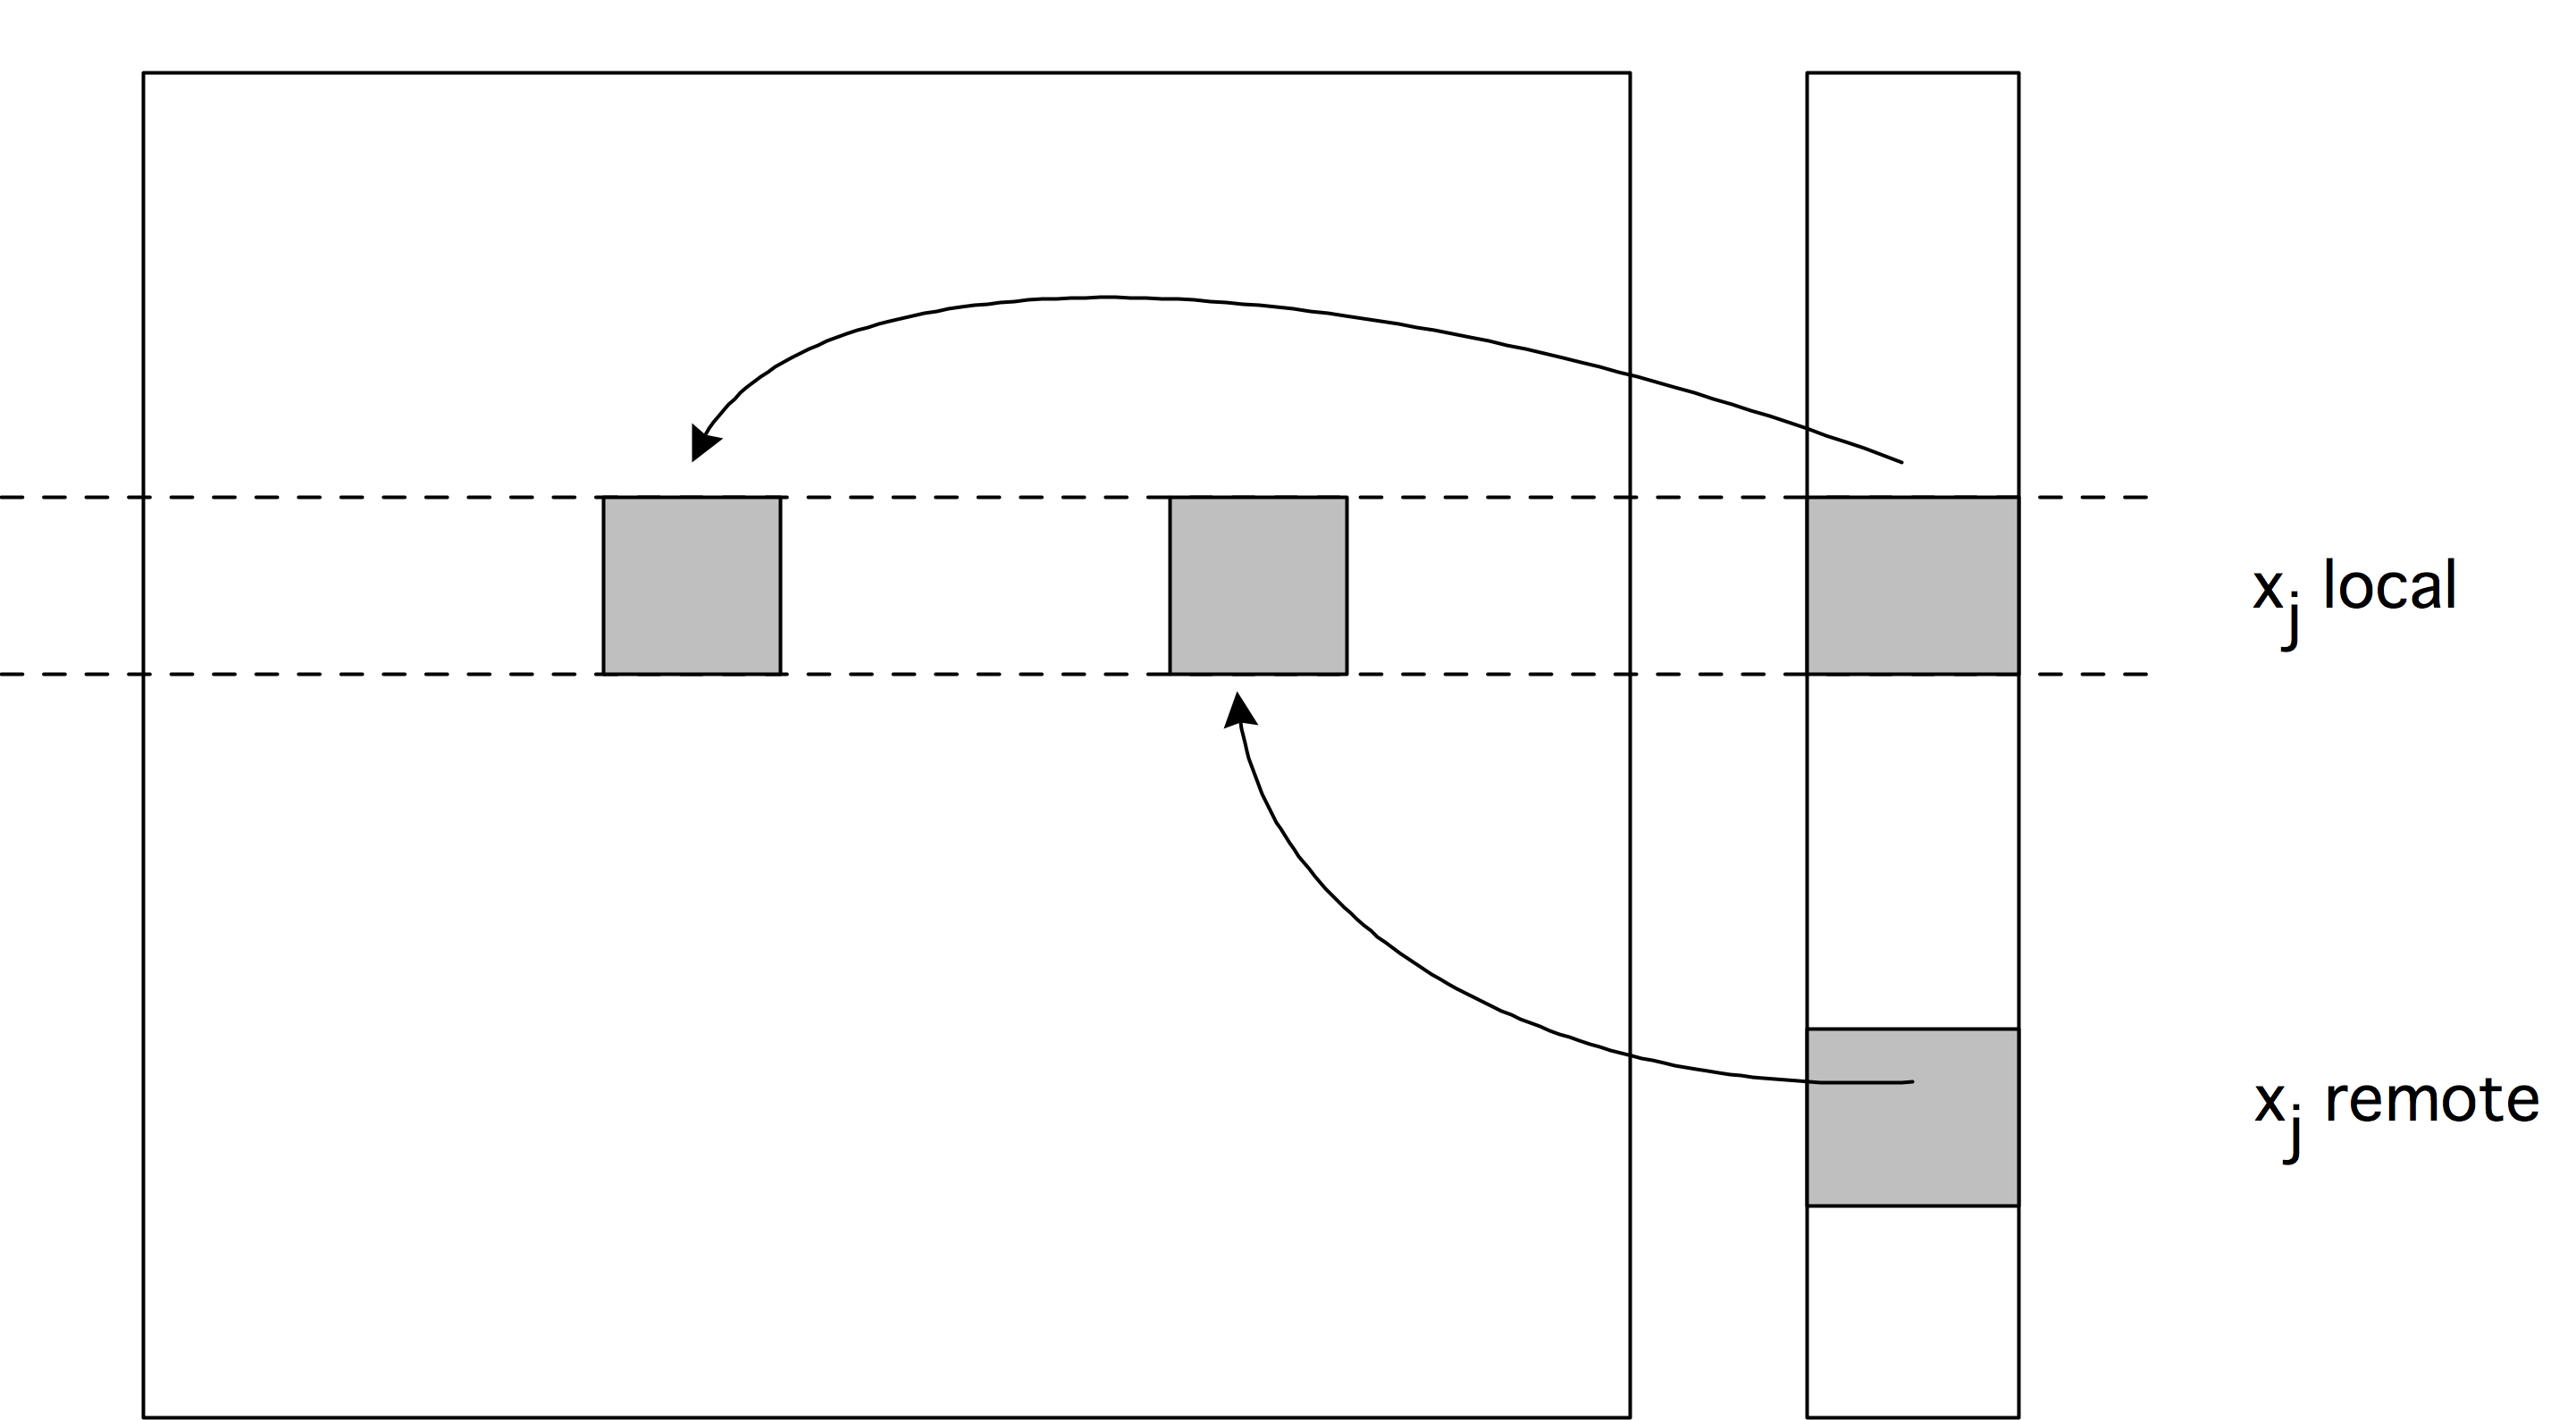
\includegraphics[scale=.12]{graphics/distmvp}
  \end{quote}
  \caption{The parallel matrix-vector product with a blockrow
    distribution.}
  \label{fig:distmvp2}
\end{figure}
figure~\ref{fig:distmvp2} for an illustration.) The parallel algorithm
is given in figure~\ref{fig:buffer-pmvp}.
\begin{figure}
\begin{displayprocedure}{Parallel MVP}{$A,x\sublocal,y\sublocal,p$}
  \KwIn{Processor number~$p$; the elements $x_i$ with $i\in I_p$; matrix
    elements $A_{ij}$ with $i\in I_p$.}
  \KwOut{The elements $y_i$ with $i\in I_p$}
  \For{$q\not=p$}{Send elements of~$x$ from processor $q$ to~$p$,
    receive in buffer~$B_{pq}$.}
  $y\sublocal\leftarrow A x\sublocal$\\
  \For{$q\not=p$}{$y\sublocal\leftarrow y\sublocal+A_{pq}B_q$}
\end{displayprocedure}
  \caption{A buffered implementation of the parallel matrix-vector
    product}
  \label{fig:buffer-pmvp}
\end{figure}

In addition to preventing an element from being fetched more than
once, this also combines many small messages into one large message,
which is usually more efficient; recall our discussion of bandwidth
and latency in section~\ref{sec:bwlatency}.

\begin{exercise}
  Give pseudocode for the matrix-vector product using 
  nonblocking operations (section~\ref{sec:nonblocking})
\end{exercise}

Above we said that having a copy of the whole of~$x$ on each processor
was wasteful in space. The implicit argument here is that, in general,
we do not want local storage to be function of the number of
processors: ideally it should be only a function of the local
data. (This is related to weak scaling; section~\ref{sec:scaling}.)

You see that, because of communication considerations, we have
actually decided that it is unavoidable, or at least preferable, for
each processor to store the whole input vector.  Such trade-offs
between space and time efficiency are fairly common in parallel
programming. For the dense matrix-vector product we can actually
defend this overhead, since the vector storage is of lower order than
the matrix storage, so our over-allocation is small by ratio. Below
(section~\ref{sec:pspmvp}), we will see that for the sparse
matrix-vector product the overhead can be much less.

It is easy to see that the parallel dense matrix-vector product, as
described above, has perfect speedup \emph{if we are allowed to ignore
the time for communication}. In the next couple of sections you will
see that the block row implementation above is not optimal if we take
communication into account. For scalability we need a two-dimensional
decomposition. We start with a discussion of collectives.

\Level 1 {Scalability of the dense matrix-vector product}
\label{sec:densescaling}

\input chapters/robertmacros

In this section, we will give a full analysis of the parallel
computation of $ y \becomes A x $, where $ x, y \in \Rn $ and $ A \in
\Rnxn $.  We will assume that $ p $ nodes will be used, but we make no
assumptions on their connectivity. We will see that the way the matrix
is distributed makes a big difference for the scaling of the
algorithm; for the original research
see~\cite{HeWo:94,Schreiber:scalability92,Stewart90}, and see
section~\ref{sec:scaling} for the definitions of the various forms of
scaling.

\Level 2 {Matrix-vector product, partitioning by rows}
\label{sec:mvp-by-rows}

Partition
\[
A \rightarrow \defcolvector{A}{p} 
\quad
x \rightarrow \defcolvector{x}{p} ,
\quad
\mbox{and}
\quad
y \rightarrow \defcolvector{y}{p} ,
\]
where $ A_i \in \R^{m_i \times n} $ and $ x_i, y_i \in \R^{m_i} $ with
$ \sum_{i=0}^{p-1} m_i = n $ and $ m_i \approx n / p $.
We will start by assuming
that $ A_i $, $ x_i $, and $ y_i $ are originally assigned to $ {\cal P}_i $.

The computation is characterized by the fact that each processor needs
the whole vector~$x$, but owns only an $n/p$ fraction of it. Thus, we
execute an \indexterm{allgather} of~$x$. After this, the processor can
execute the local product $y_i\becomes A_ix$; no further communication
is needed after that.

An algorithm with cost computation
for $ y = A x $ in parallel is then given by

\[ \vcenter{\hskip\unitindent
\setbox0=\hbox{Allgather $ x_i $ so that $ x $ is available on all nodes
}
\dimen0=\wd0
\setbox1=\hbox{$ \lceil \log_2(p)\rceil \alpha + \frac{p-1}{p} n \beta$ }
\dimen1=\wd1
\begin{tabular}{| p{\dimen0} |  p{\dimen1} |}\hline
Step & Cost (lower bound) \\ \whline
Allgather $ x_i $ so that $ x $ is available on all nodes & 
$ \lceil \log_2(p)\rceil \alpha + \frac{p-1}{p} n \beta$\\
&$ \approx \log_2(p) \alpha + n \beta $ \\
Locally compute $ y_i = A_i x $ &
$ \approx 2 \frac{n^2}{p} \gamma $ \\ \hline
\end{tabular}
}
\]

\paragraph*{Cost analysis}

The total cost of the algorithm is given by, approximately,
\[
T_p(n) = T_p^{\mbox{1D-row}}(n) = 
2 \frac{n^2}{p} \gamma + 
\begin{array}[t]{c}
\underbrace{\log_2(p) \alpha + n \beta.}
\\
\mbox{Overhead}
\end{array}
\]
Since the sequential cost is $ T_1(n) = 2 n^2 \gamma $, the speedup is given by
\[
S_p^{\mbox{1D-row}}(n) = 
\frac{T_1(n)}
{T_p^{\mbox{1D-row}}(n)} = 
\frac{2 n^2 \gamma}
{ 2 \frac{n^2}{p} \gamma + 
\log_2(p) \alpha + n \beta}
= 
\frac{p}
{ 1 + \frac{p \log_2(p)}{2 n^2} \frac{\alpha}{\gamma} 
+ \frac{p}{2 n} \frac{\beta}{\gamma} }
\]
and the parallel efficiency by
\[
E_p^{\mbox{1D-row}}(n) = 
\frac{S_p^{\mbox{1D-row}}(n)}{p}
= 
\frac{1}
{ 1 + \frac{p \log_2(p)}{2 n^2} \frac{\alpha}{\gamma} 
+ \frac{p}{2 n} \frac{\beta}{\gamma} }.
\]

\paragraph*{An optimist's view}

Now, if one fixes $ p $ and lets $ n $ get large,
\[
\lim_{n \rightarrow \infty} E_p( n ) =
\lim_{n \rightarrow \infty}
\left[
\frac{1}
{ 1 + \frac{p \log_2(p)}{2 n^2} \frac{\alpha}{\gamma} 
+ \frac{p}{2 n} \frac{\beta}{\gamma} }
\right]
=
1.
\]
Thus, if one can make the problem large enough, eventually the parallel
efficiency is nearly perfect. However, this assumes unlimited memory,
so this analysis is not practical.



\paragraph*{A pessimist's view}

In a \indextermsub{strong}{scalability} analysis,
one fixes $ n $ and lets $ p $ get large, to get
\[
\lim_{p \rightarrow \infty} E_p( n ) =
\lim_{p \rightarrow \infty}
\left[
\frac{1}
{1 + \frac{p \log_2(p)}{2 n^2} \frac{\alpha}{\gamma} 
+ \frac{p}{2 n} \frac{\beta}{\gamma} }
\right]
=
0.
\]
Thus, eventually the parallel efficiency becomes nearly nonexistent.

\paragraph*{A realist's view}

In a more realistic view we increase the number of processors with the
amount of data. This is called \indextermsub{weak}{scalability}, and 
it makes the amount of memory that is available to
store the problem scale linearly with~$ p $.  

Let $ M $ equal the
number of floating point numbers that can be stored in a single node's
memory.  Then the aggregate memory is given by $ M p $.  Let $
n_{\max}(p) $ equal the largest problem size that can be stored
in the aggregate memory of $ p $ nodes.  Then, if {\em all} memory can
be used for the matrix,
\[
(n_{\max}(p))^2 = M p
\quad
\mbox{or}
\quad
n_{\max}(p) = \sqrt{Mp}.
\]
The question now becomes what the parallel 
efficiency for the largest problem that can be stored on $ p $ nodes:
\[ 
\begin{array}{r@{{}={}}l}
E_p^{\mbox{1D-row}}(n_{\max}(p)) &
\frac{1}
{1 + \frac{p \log_2(p)}{2 (n_{\max}(p))^2} \frac{\alpha}{\gamma} 
+ \frac{p}{2 n_{\max}(p)} \frac{\beta}{\gamma} }
\\
&
\frac{1}
{ 1 + \frac{\log_2(p)}{2 M} \frac{\alpha}{\gamma} 
+ \frac{\sqrt{p}}{2 \sqrt{M}} \frac{\beta}{\gamma} }.
\end{array}
\]
Now, if one analyzes what happens when the number of nodes
becomes large, one finds that
\[
\lim_{p \rightarrow \infty} E_p( n_{\max}(p) ) 
=
\lim_{p \rightarrow \infty}
\left[
\frac{1}
{1 + \frac{\log_2(p)}{2 M} \frac{\alpha}{\gamma} 
+ \frac{\sqrt{p}}{2 \sqrt{M}} \frac{\beta}{\gamma} }
\right]
=
0.
\]
Thus, this parallel algorithm for matrix-vector multiplication does
not scale. 

If you take a close look at this expression for efficiency,
you'll see that the main problem is the $1/\sqrt p$ part of the
expression. This terms involves a factor~$\beta$, and if you follow
the derivation backward you see that it comes from the time to send
data between the processors. Informally this can be described as
saying that the message size is too large to make the problem
scalable. In fact, the message size is constant~$n$, regardless the
number of processors.

Alternatively, a realist realizes that there is a limited amount of time,
$ T_{\max} $, to get a computation done.
Under the best of circumstances, 
that is, with zero communication overhead, the largest problem
that we can solve in time $ T_{\max} $ is given by
\[ 
T_p(n_{\max}(p)) = 2 \frac{(n_{\max}(p))^2}{p} \gamma = T_{\max} .
\]
Thus
\[
(n_{\max}(p))^2 = \frac{T_{\max} p}{2 \gamma}
\quad
\mbox{or}
\quad
n_{\max}(p) = \frac{\sqrt{T_{\max}} \sqrt{p}}{\sqrt{2 \gamma}}.
\]
Then the parallel efficiency that is attained by the algorithm for the largest
problem that can be solved in time $ T_{\max} $ is given by
\[
  E_{p,n_{\max}}=\frac1
  {1+\frac{\log_2p}T\alpha+\sqrt{\frac pT\frac \beta\gamma}}
\]
and the parallel efficiency as the number of nodes becomes large approaches
\[
\lim_{p\rightarrow\infty}E_p= \sqrt{\frac{T\gamma}{p\beta}}.
\]
Again, efficiency cannot be maintained as the number of processors
increases and the execution time is capped.

\Level 2 {Matrix-vector product, partitioning by columns}

Partition
\[
A \rightarrow \defrowvector{A}{p} 
\quad
x \rightarrow \defcolvector{x}{p} ,
\quad
\mbox{and}
\quad
y \rightarrow \defcolvector{y}{p} ,
\]
where $ A_j \in \R^{n \times n_j} $ and $ x_j, y_j \in \R^{n_j} $ with
$ \sum_{j=0}^{p-1} n_j = n $ and $ n_j \approx n / p $.

We will start by assuming that $ A_j $, $ x_j $, and $ y_j $ are
originally assigned to $ {\cal P}_j $ (but now $ A_i $ is a block of
columns). In this algorithm by columns, processor~$i$ can compute the
length~$n$ vector $A_ix_i$ without prior communication. These partial
results then have to be added together
\[ y\leftarrow \sum_i A_ix_i \]
in a \indexterm{reduce-scatter} operation: each processor~$i$ scatters
a part $(A_ix_i)_j$ of its result to processor~$j$. The receiving
processors then perform a reduction, adding all these fragments: 
\[ y_j = \sum_i (A_ix_i)_j. \]

The algorithm with costs is then given by:

\[ \vcenter{\hskip\unitindent
\setbox0=\hbox{Reduce-scatter the $ y^{(j)} $s so that $ y_i = \sum_{j=0}^{p-1}
y_i^{(j)} $ is on $ {\cal P}_i $ }
\dimen0=\wd0
\setbox1=\hbox{$ \lceil \log_2(p)\rceil \alpha + \frac{p-1}{p} n \beta
+ \frac{p-1}{p} n \gamma $ }
\dimen1=\wd1
\begin{tabular}{| p{\dimen0} |  p{\dimen1} |}\hline
Step & Cost (lower bound) \\ \whline
Locally compute $ y^{(j)} = A_j x_j $ &
$ \approx 2 \frac{n^2}{p} \gamma $ \\ 
Reduce-scatter the $ y^{(j)} $s so that $ y_i = \sum_{j=0}^{p-1}
y_i^{(j)} $ is on $ {\cal P}_i $ & 
$ \lceil \log_2(p)\rceil \alpha + \frac{p-1}{p} n \beta
+ \frac{p-1}{p} n \gamma $\\
& $ \approx \log_2(p) \alpha + n ( \beta + \gamma ) $ \\
\hline
\end{tabular}
}
\]

\paragraph*{Cost analysis}

The total cost of the algorithm is given by, approximately,
\[
T_p^{\mbox{1D-col}}(n) = 
2 \frac{n^2}{p} \gamma + 
\begin{array}[t]{c}
\underbrace{\log_2(p) \alpha + n ( \beta + \gamma ).}
\\
\mbox{Overhead}
\end{array}
\]
Notice that this is identical to the cost  
$ T_p^{\mbox{1D-row}}(n)  $, except with $ \beta $ replaced by $ (\beta + \gamma )$.  It is not hard to see that the conclusions about scalability 
are the same.


\Level 2 {Two-dimensional partitioning}
\label{sec:mvp-2d}

Next,
partition
\[
A \rightarrow \defmatrix{A}{p}{p}
\quad
x \rightarrow \defcolvector{x}{p} ,
\quad
\mbox{and}
\quad
y \rightarrow \defcolvector{y}{p} ,
\]
where $ A_{ij} \in \R^{n_i \times n_j} $ and $ x_i, y_i \in \R^{n_i} $ with
$ \sum_{i=0}^{p-1} n_i = N $ and $ n_i \approx N / \sqrt P $.

We will view the nodes as an $ r \times c $ mesh, with $ P = r c $,
and index them as $p_{ij}$, 
%
with $ i=0, \ldots, r-1 $ and $ j = 0,\ldots, c-1 $.
%
Figure~\ref{fig:2dmatrix}, for a $12\times12$ matrix
on a $3\times4$ processor grid,
illustrates the assignment of data to nodes, where the $ i,j$
`cell' shows the matrix and vector elements owned by  $ p_{ij} $.

\begin{figure}[ht]
{\footnotesize
\[
\begin{array}{| c | c | c | c |} \hline
% 0,0
\begin{array}{c c c c}
x_0\\
a_{00} & a_{01} &a_{02} & y_0\\
a_{10} & a_{11} &a_{12} & \\
a_{20} & a_{21} &a_{22} & \\
a_{30} & a_{31} &a_{32} & \\
\end{array}
&
% 0,1
\begin{array}{c c c c}
x_3\\
a_{03} & a_{04} &a_{05} & \\
a_{13} & a_{14} &a_{15} & y_1\\
a_{23} & a_{24} &a_{25} & \\
a_{33} & a_{34} &a_{35} & \\
\end{array}
&
% 0,2
\begin{array}{c c c c}
x_6\\
a_{06} & a_{07} &a_{08} & \\
a_{16} & a_{17} &a_{18} & \\
a_{26} & a_{27} &a_{28} & y_2 \\
a_{37} & a_{37} &a_{38} & \\
\end{array}
&
% 0,3
\begin{array}{c c c c}
x_9\\
a_{09} & a_{0,10} & a_{0,11} & \\
a_{19} & a_{1,10} & a_{1,11} & \\
a_{29} & a_{2,10} & a_{2,11} & \\
a_{39} & a_{3,10} & a_{3,11} & y_3 \\
\end{array}
\\ \hline
% 1,0
\begin{array}{c c c c}
& x_1\\
a_{40} & a_{41} &a_{42} & y_4\\
a_{50} & a_{51} &a_{52} & \\
a_{60} & a_{61} &a_{62} & \\
a_{70} & a_{71} &a_{72} & \\
\end{array}
&
% 1,1
\begin{array}{c c c c}
& x_4\\
a_{43} & a_{44} &a_{45} & \\
a_{53} & a_{54} &a_{55} & y_5\\
a_{63} & a_{64} &a_{65} & \\
a_{73} & a_{74} &a_{75} & \\
\end{array}
&
% 1,2
\begin{array}{c c c c}
& x_7\\
a_{46} & a_{47} &a_{48} & \\
a_{56} & a_{57} &a_{58} & \\
a_{66} & a_{67} &a_{68} & y_6 \\
a_{77} & a_{77} &a_{78} & \\
\end{array}
&
% 1,3
\begin{array}{c c c c}
& x_{10}\\
a_{49} & a_{4,10} & a_{4,11} & \\
a_{59} & a_{5,10} & a_{5,11} & \\
a_{69} & a_{6,10} & a_{6,11} & \\
a_{79} & a_{7,10} & a_{7,11} & y_7 \\
\end{array}
\\ \hline
% 0,0
\begin{array}{c c c c}
&&x_2\\
a_{80} &  a_{81} &  a_{82} & y_8\\
a_{90} &  a_{91}   &a_{92} & \\
a_{10,0} &a_{10,1} &a_{10,2} & \\
a_{11,0} &a_{11,1} &a_{11,2} & \\
\end{array}
&
% 0,1
\begin{array}{c c c c}
&&x_5\\
a_{83} &   a_{84} &  a_{85} & \\
a_{93} &   a_{94} &  a_{95} & y_9\\
a_{10,3} & a_{10,4} &a_{10,5} & \\
a_{11,3} & a_{11,4} &a_{11,5} & \\
\end{array}
&
% 0,2
\begin{array}{c c c c}
&&x_8\\
a_{86} &   a_{87} &  a_{88} & \\
a_{96} &   a_{97} &  a_{98} & \\
a_{10,6} & a_{10,7} &a_{10,8} & y_{10} \\
a_{11,7} & a_{11,7} &a_{11,8} & \\
\end{array}
&
% 0,3
\begin{array}{c c c c}
&&x_{11}\\
a_{89} &   a_{8,10} &  a_{8,11} & \\
a_{99} &   a_{9,10} &  a_{9,11} & \\
a_{10,9} & a_{10,10} & a_{10,11} & \\
a_{11,9} & a_{11,10} & a_{11,11} & y_{11} \\
\end{array}
\\ \hline
\end{array}
\]
}
\caption{Distribution of matrix and vector elements for a problem of size 12 on a $4\times 3$ processor grid}
\label{fig:2dmatrix}
\end{figure}

In other words, $ p_{ij} $ owns the matrix block $A_{ij}$
and parts of $x$ and~$y$. This makes possible the following algorithm\footnote
{This figure shows a partitioning of the matrix into contiguous blocks,
and the vector distribution seem to be what is necessary to work with this 
matrix distribution. You could also look at this story the other way:
start with a distribution of input and output vector, and then decide what
that implies for the matrix distribution. For instance, if you distributed
$x$ and~$y$ the same way, you would arrive at a different matrix distribution,
but otherwise the product algorithm would be much the same; see~\cite{Flame:PBMD-report}.}:
\begin{itemize}
\item Since $x_j$ is distributed over the $j$th column, the algorithm starts
  by collecting $x_j$ on each processor $p_{ij}$ by an
  \indexterm{allgather} inside the processor columns.
\item Each processor $p_{ij}$ then computes $y_{ij} = A_{ij}x_j$. This
  involves no further communication.
\item The result $y_i$ is then collected by gathering together the
  pieces $y_{ij}$ in each processor row to form~$y_i$, and this is then
  distributed over the processor row. These two operations are in fact
  combined to form a \indexterm{reduce-scatter}.
\item If $r=c$, we can transpose the $y$ data over the processors, so
  that it can function as the input for a subsequent matrix-vector
  product. If, on the other hand, we are computing $A^tAx$, then $y$
  is now correctly distributed for the $A^t$ product.
\end{itemize}


\paragraph*{Algorithm}

The algorithm with cost analysis is
\[ \vcenter{\hskip\unitindent
\setbox0=\hbox{Perform local matrix-vector multiply }
\dimen0=\wd0
\setbox1=\hbox{$ \lceil \log_2(c)\rceil \alpha + \frac{c-1}{p} n \beta +
\frac{c-1}{p} n \gamma $ }
\dimen1=\wd1
\begin{tabular}{| p{\dimen0} |  p{\dimen1} |}\hline
Step & Cost (lower bound) \\ \whline
Allgather $ x_i $'s  within columns & 
$ \lceil \log_2(r)\rceil \alpha + \frac{r-1}{p} n \beta$\\
& $ \approx \log_2(r) \alpha + \frac{n}{c} \beta $ \\
Perform local matrix-vector multiply &
$ \approx 2 \frac{n^2}{p} \gamma $ \\ 
Reduce-scatter $ y_i $'s  within rows & 
$ \lceil \log_2(c)\rceil \alpha + \frac{c-1}{p} n \beta +
\frac{c-1}{p} n \gamma $\\
& $ \approx \log_2(c) \alpha + \frac{n}{c} \beta + \frac{n}{c} \gamma
$ \\ 
\hline
\end{tabular}
}
\]

\paragraph*{Cost analysis}

The total cost of the algorithm is given by, approximately,
\[
T_p^{r \times c}(n) = T_p^{r \times c}( n) = 
2 \frac{n^2}{p} \gamma + 
\begin{array}[t]{c}
\underbrace{\log_2(p) \alpha + \left( \frac{n}{c} + \frac{n}{r} \right) \beta + \frac{n}{r} \gamma.}
\\
\mbox{Overhead}
\end{array}
\]
We will now make the simplification that $ r = c = \sqrt{p} $ so that
\[
T_p^{\sqrt{p} \times \sqrt{p}}(n) = T_p^{\sqrt{p} \times \sqrt{p}}( n) = 
2 \frac{n^2}{p} \gamma + 
\begin{array}[t]{c}
\underbrace{\log_2(p) \alpha + \frac{n}{\sqrt{p}}\left( 2 \beta+ \gamma \right) 
}
\\
\mbox{Overhead}
\end{array}
\]

Since the sequential cost is $ T_1(n) = 2 n^2 \gamma $, the speedup is given by
\[
S_p^{\sqrt{p} \times \sqrt{p}}(n) = 
\frac{T_1(n)}
{T_p^{\sqrt{p} \times \sqrt{p}}(n)} = 
\frac{2 n^2 \gamma}
{ 2 \frac{n^2}{p} \gamma + \frac{n}{\sqrt{p}}
\left( 2 \beta + \gamma \right)}
= 
\frac{p}
{ 1 + \frac{p \log_2(p)}{2 n^2} \frac{\alpha}{\gamma} 
+ \frac{\sqrt{p}}{2n}\frac{
\left( 2 \beta + \gamma \right)}{\gamma}}
\]
and the parallel efficiency by
\[
E_p^{\sqrt{p} \times \sqrt{p}}(n) = 
\frac{1}
{ 1 + \frac{p \log_2(p)}{2 n^2} \frac{\alpha}{\gamma} 
+ \frac{\sqrt{p}}{2n}\frac{
\left( 2 \beta + \gamma \right)}{\gamma}}
\]

We again ask the question what the parallel 
efficiency for the largest problem that can be stored on $ p $ nodes is.
\begin{eqnarray*}
E_p^{\sqrt{p} \times \sqrt{p}}(n_{\max}(p)) &=& 
\frac{1}
{ 1 + \frac{p \log_2(p)}{2 n^2} \frac{\alpha}{\gamma} 
+ \frac{\sqrt{p}}{2n}\frac{
\left( 2 \beta + \gamma \right)}{\gamma}}
\\
&=&
\frac{1}
{ 1 + \frac{\log_2(p)}{2 M} \frac{\alpha}{\gamma} 
+ \frac{1}{2\sqrt{M}}\frac{
\left( 2 \beta + \gamma \right)}{\gamma}}
\end{eqnarray*}
so that still
\begin{eqnarray*}
\lim_{p \rightarrow \infty}
E_p^{\sqrt{p} \times \sqrt{p}}(n_{\max}(p)) &=& 
\lim_{p \rightarrow \infty}
\frac{1}
{ 1 + \frac{\log_2(p)}{2 M} \frac{\alpha}{\gamma} 
+ \frac{1}{2\sqrt{M}}\frac{
\left( 2 \beta + \gamma \right)}{\gamma}}
=
0.
\end{eqnarray*}
However, $ \log_2{p} $ grows very slowly with $ p $ and is therefore
considered to act much like a constant.  In this case 
$ E_p^{\sqrt{p}\times \sqrt{p}}( n_{\rm max}(p) ) $ decreases very slowly and the algorithm is considered to be scalable for practical purposes.


Note that when $ r = p $ the 2D algorithm becomes the "partitioned by
rows" algorithm and when $ c = p $ it becomes the "partitioned by
columns" algorithm.  It is not hard to show that the 2D algorithm is
scalable in the sense of the above analysis
when $ r = c $, as long as $ r / c
$ is kept constant.
%\input chapters/mvpscaling2

\Level 0 {LU factorization in parallel}

The matrix-vector and matrix-product are easy to parallelize in one sense.
The elements of the output can all be computed independently and in any order,
so we have many degrees of freedom in parallelizing the algorithm.
This does not hold for computing an LU factorization, or solving a linear system
with the factored matrix.

\Level 1 {Solving a triangular system}
\index{LU factorization!solution in parallel|(}

The solution of a triangular system $y=L\inv x$ (with $L$~is lower triangular)
is a matrix-vector operation, so
it has its $O(N^2)$ complexity in common with the matrix-vector product.
However, unlike the product operation, this solution process contains a recurrence
relation between the output elements: 
\[ y_{i} = \ell_{ii}\inv ( x_i-\sum_{j<i} \ell_{ij}x_j ). \]
This means that parallelization is not trivial.
In the case of a sparse matrix special strategies may be possible; see section~\ref{sec:parallel-implicit}.
Here we will make a few remarks about general, dense case.

Let us assume for simplicity that communication takes no time, and
that all arithmetic operations take the same unit time.
First we consider the matrix distribution by rows,
meaning that processor~$p$ stores the elements~$\ell_{p*}$.
With this we can implement the triangular solution as:
\begin{itemize}
\item Processor 1 solves $y_1=\ell_{11}\inv x_1$ and sends its value to the next processor.
\item In general, processor $p$ gets the values $y_1,\ldots,y_{p-1}$
  from processor~$p-\nobreak1$, and computes~$y_p$;
\item Each processor $p$ then sends $y_1,\ldots,y_p$ to $p+1$.
\end{itemize}

\begin{exercise}
  Show that this algorithm takes time $2N^2$, just like the sequential algorithm.
\end{exercise}

This algorithm has each processor passing all computed $y_i$ values to its successor, in a pipeline fashion.
However, this means that processor~$p$ receives~$y_1$ only at the last moment, whereas that value was computed
already in the first step. We can formulate the solution algorithm in such a way that computed elements
are made available as soon as possible:
\begin{itemize}
\item Processor~1 solve $y_1$, and sends it to all later processors.
\item In general, processor~$p$ waits for individual messages with values $y_q$ for~$q<p$.
\item Processor $p$ then computes $y_p$ and sends it to processors~$q$ with $q>p$.
\end{itemize}

Under the assumption that communication time is negligible, this algorithm can be much faster.
For instance, all processors~$p>1$ receive~$y_1$ simultaneously, and can compute $\ell_{p1}y_1$
simultaneously.

\begin{exercise}
  Show that this algorithm variant takes a time $O(N)$.
\end{exercise}

\begin{exercise}
  Now consider the matrix distribution by columns: processor~$p$ stores~$\ell_{*p}$.
  Outline the triangular solution algorithm with this distribution, and show that the
  parallel solve time is~$O(N)$.
\end{exercise}

\index{LU factorization!solution in parallel|)}

\Level 1 {Factorization}
\index{LU factorization!computation in parallel|(}
\label{sec:LUscaling}

A full analysis of the scalability of dense LU factorization is quite
involved, so we will state without further proof that as in the matrix-vector case a
two-dimensional distribution is needed. However, we can identify a
further complication. Since factorizations of any
type\footnote{Gaussian elimination can be performed in right-looking,
  left-looking and Crout variants; see~\cite{TSoPMC}.}
progress through a matrix, processors will be inactive for part of the
time.

\begin{exercise}
  Consider the regular right-looking Gaussian elimination
\begin{verbatim}
for k=1..n
  p = 1/a(k,k)
  for i=k+1,n
    for j=k+1,n
      a(i,j) = a(i,j)-a(i,k)*p*a(k,j)
\end{verbatim}
  Analyze the running time, speedup, and efficiency as a function
  of~$N$, if we assume a one-dimensional distribution, and enough
  processors to store one column per processor. Show that speedup is
  limited.

  Also perform this analysis for a two-dimensional decomposition where
  each processor stores one element.
\end{exercise}

\index{matrix!storage, dense|(}

For this reason, an \indexterm{overdecomposition} is used, where
the matrix is divided in more blocks than there are processors,
and each processor stores several, non-contiguous, sub-matrices. 
\begin{figure}[ht]
  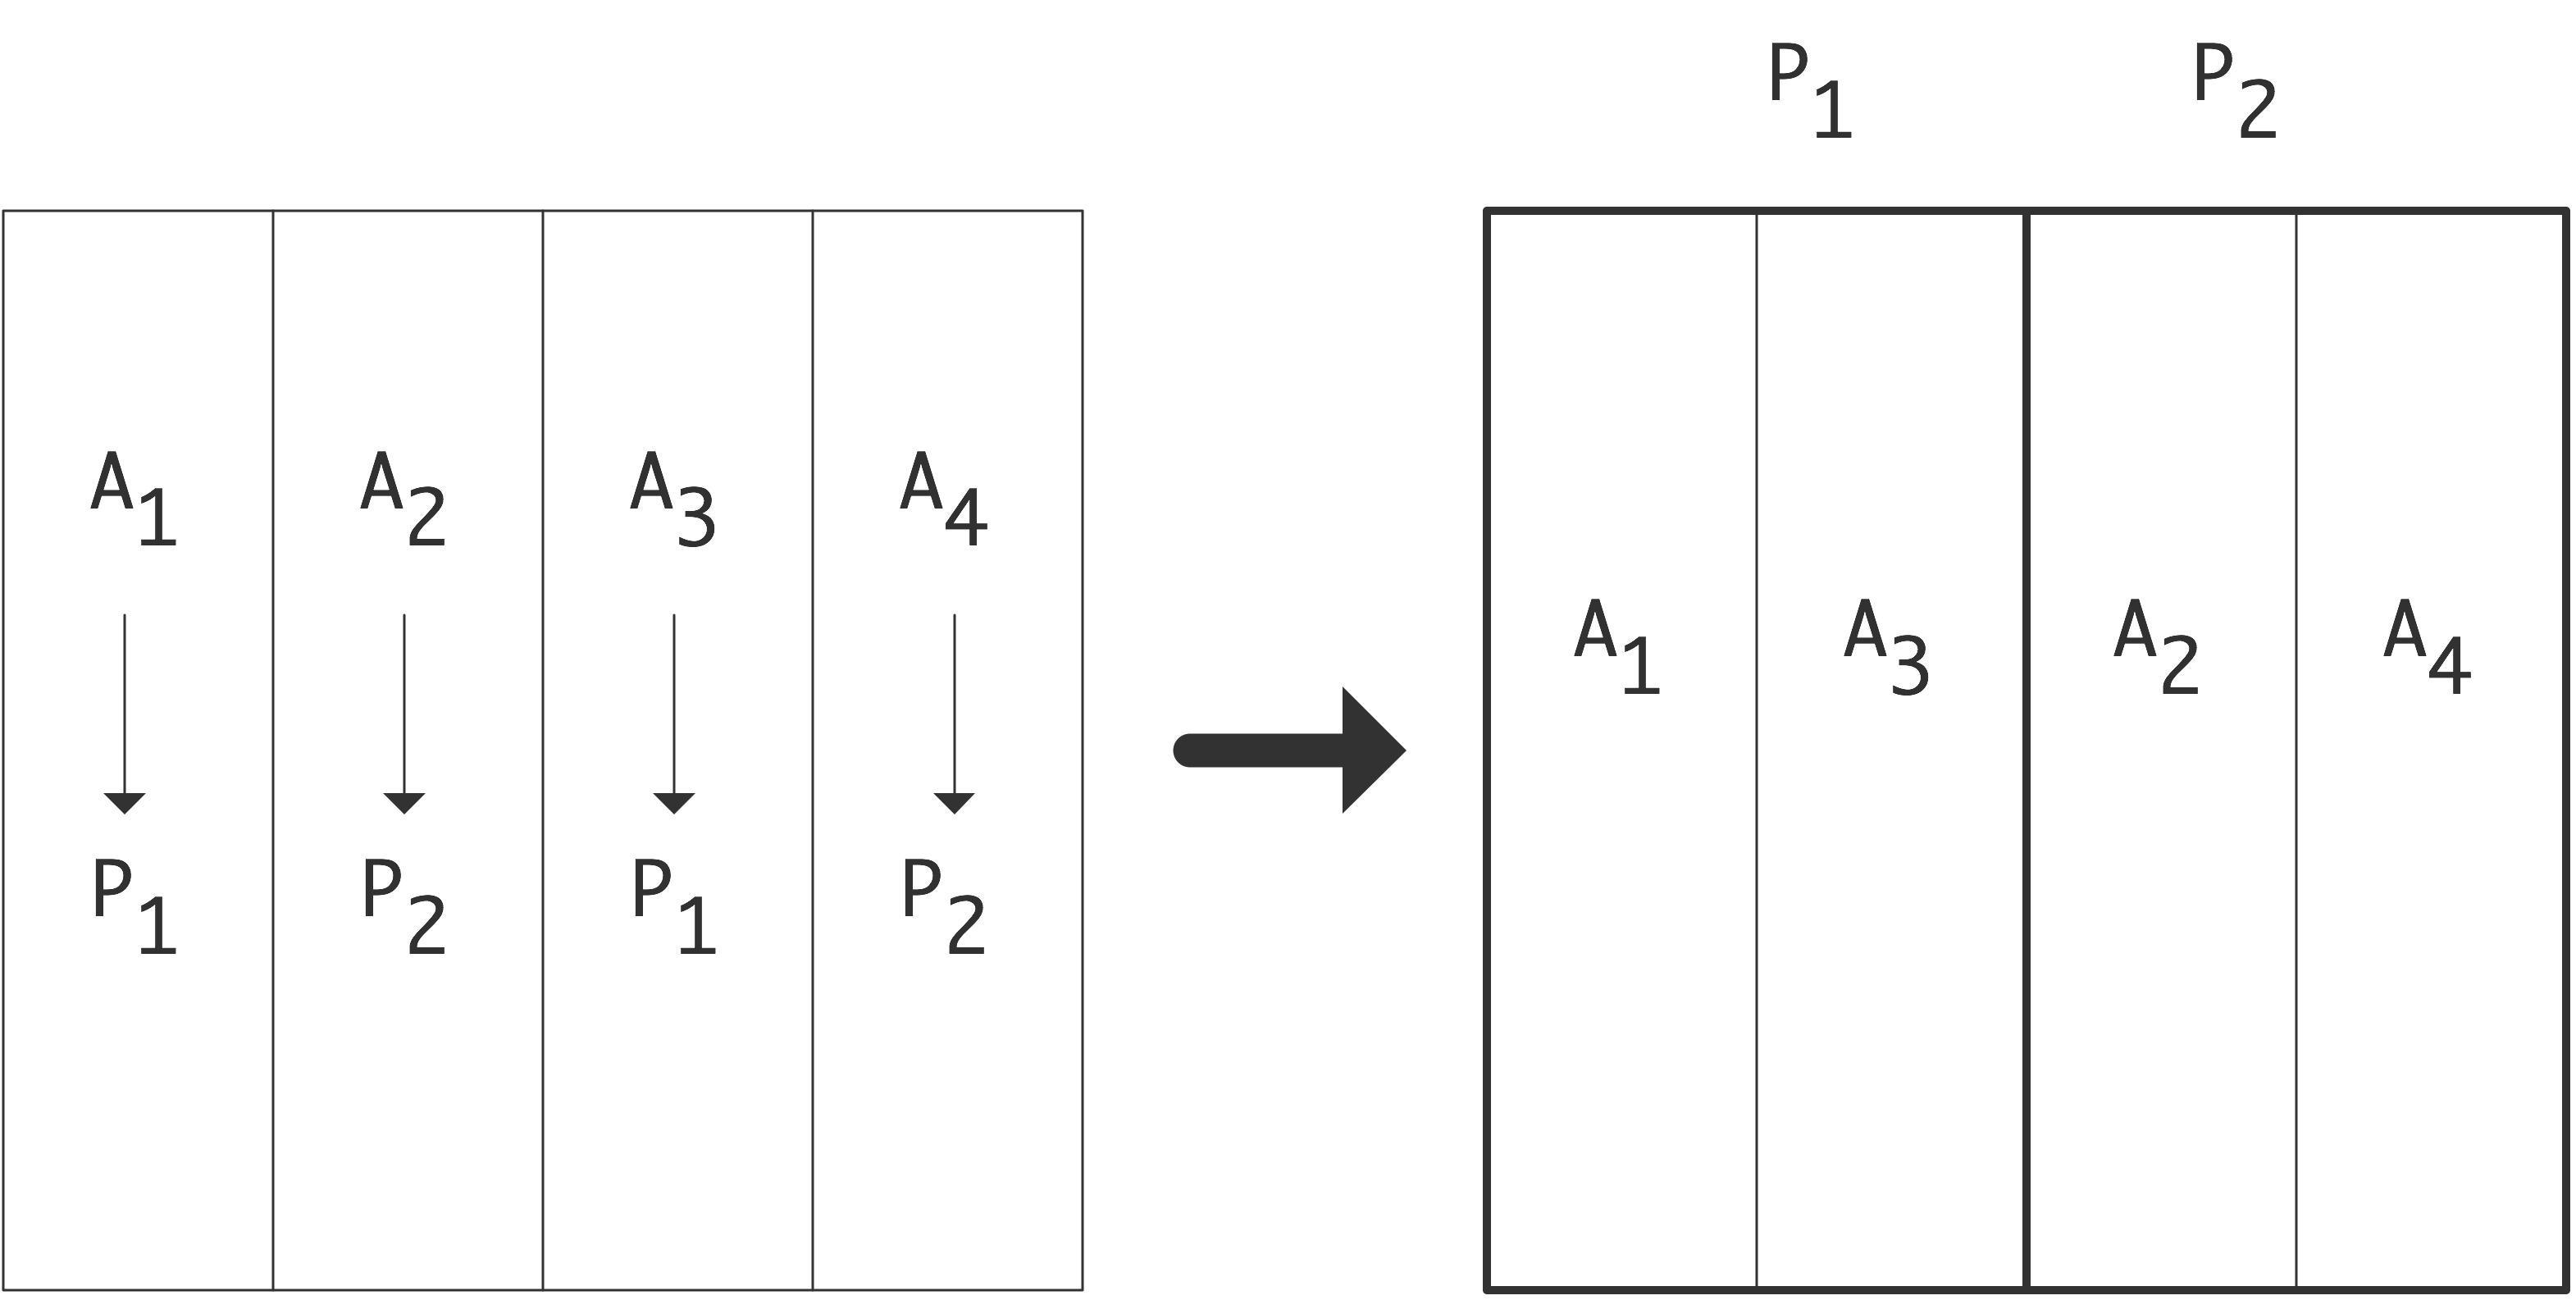
\includegraphics[scale=.11]{graphics/cyclic-1}
  \caption{One-dimensional cyclic distribution: assignment of four
    matrix columns to two processors, and the resulting mapping of
    storage to matrixcolumns}
  \label{fig:cyclic-1}
\end{figure}
We illustrate this in figure~\ref{fig:cyclic-1} where we divide four
block columns of a matrix to two processors: each processor stores in
a contiguous block of memory two non-contiguous matrix columns.

Next, we illustrate in figure~\ref{fig:cyclic-1-mvp}
\begin{figure}[ht]
  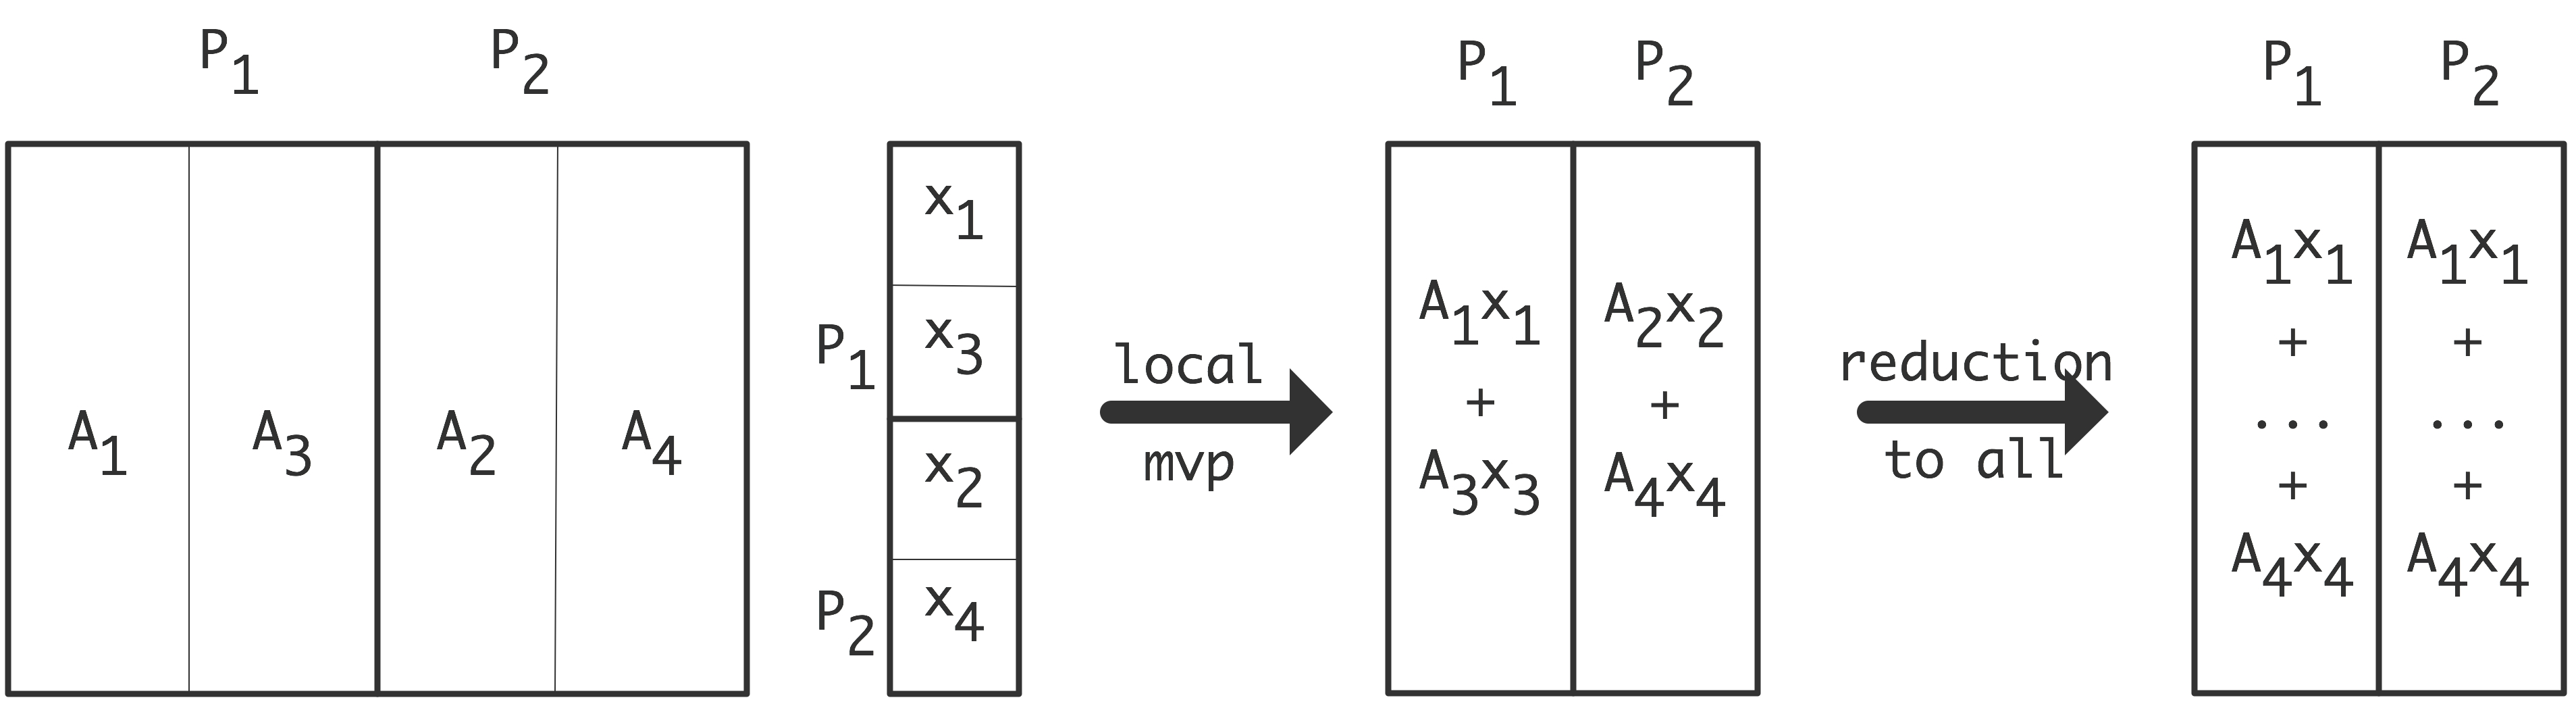
\includegraphics[scale=.11]{graphics/cyclic-1-mvp}
  \caption{Matrix-vector multiplication with a cyclicly distributed matrix}
  \label{fig:cyclic-1-mvp}
\end{figure}
that a matrix-vector product with such a matrix can be performed
without knowing that the processors store non-contiguous parts of the
matrix. All that is needed is that the input vector is also cyclicly
distributed.

\begin{exercise}
  Now consider a $4\times4$ matrix and a $2\times2$ processor
  grid. Distribute the matrix cyclicly both by rows and columns. Show
  how the matrix-vector product can again be performed using the
  contiguous matrix storage, as long as the input is distributed
  correctly. How is the output distributed? Show that more
  communication is needed than the reduction of the one-dimensional
  example.
\end{exercise}

Specifically,
with $P<N$ processors, and assuming for simplicity $N=cP$, we let
processor~0 store rows $0,c,2c,3c,\ldots$; processor~1 stores rows
$1,c+1,2c+1,\ldots$, et cetera. This scheme can be generalized two a
two-dimensional distribution, if $N=c_1P_1=c_2P_2$
and~$P=P_1P_2$. This is called a 2D \indexterm{cyclic
  distribution}. This scheme can be further extended by considering
block rows and colums (with a small block size), and assigning to
processor~0 the \emph{block} rows $0,c,2c,\ldots$.

\begin{exercise}
  Consider a square $n\times n$ matrix, and a square $p\times p$
  processor grid, where $p$ divides~$n$ without remainder. Consider
  the overdecomposition outlined above, and make a sketch of matrix
  element assignment for the specific case $n=6,p=2$. That is, draw an
  $n\times n$ table where location $(i,j)$ contains the processor
  number that stores the corresponding matrix element. Also make a
  table for each of the processors describing the local to global mapping,
  that is, giving the global $(i,j)$ coordinates of the elements in
  the local matrix. (You will find this task facilitated by using
  zero-based numbering.)

  Now write functions $P,Q,I,J$ of $i,j$ that describe the global to
  local mapping, that is, matrix element $a_{ij}$ is stored in
  location $(I(i,j),J(i,j))$ on processor $(P(i,j),Q(i,j))$.
\end{exercise}

\index{matrix!storage, dense|)}

\index{LU factorization!computation in parallel|)}

\Level 0 {Matrix-matrix product}
\index{Cannon's algorithm|see{matrix-matrix product, Cannon's algorithm}}

In section~\ref{sec:goto-gemm} we considered the high performance
implementation of the single-processor \indexterm{matrix-matrix
  product}.  We will now briefly consider the distributed memory
version of this operation.

\begin{wrapfigure}{r}{4in}
  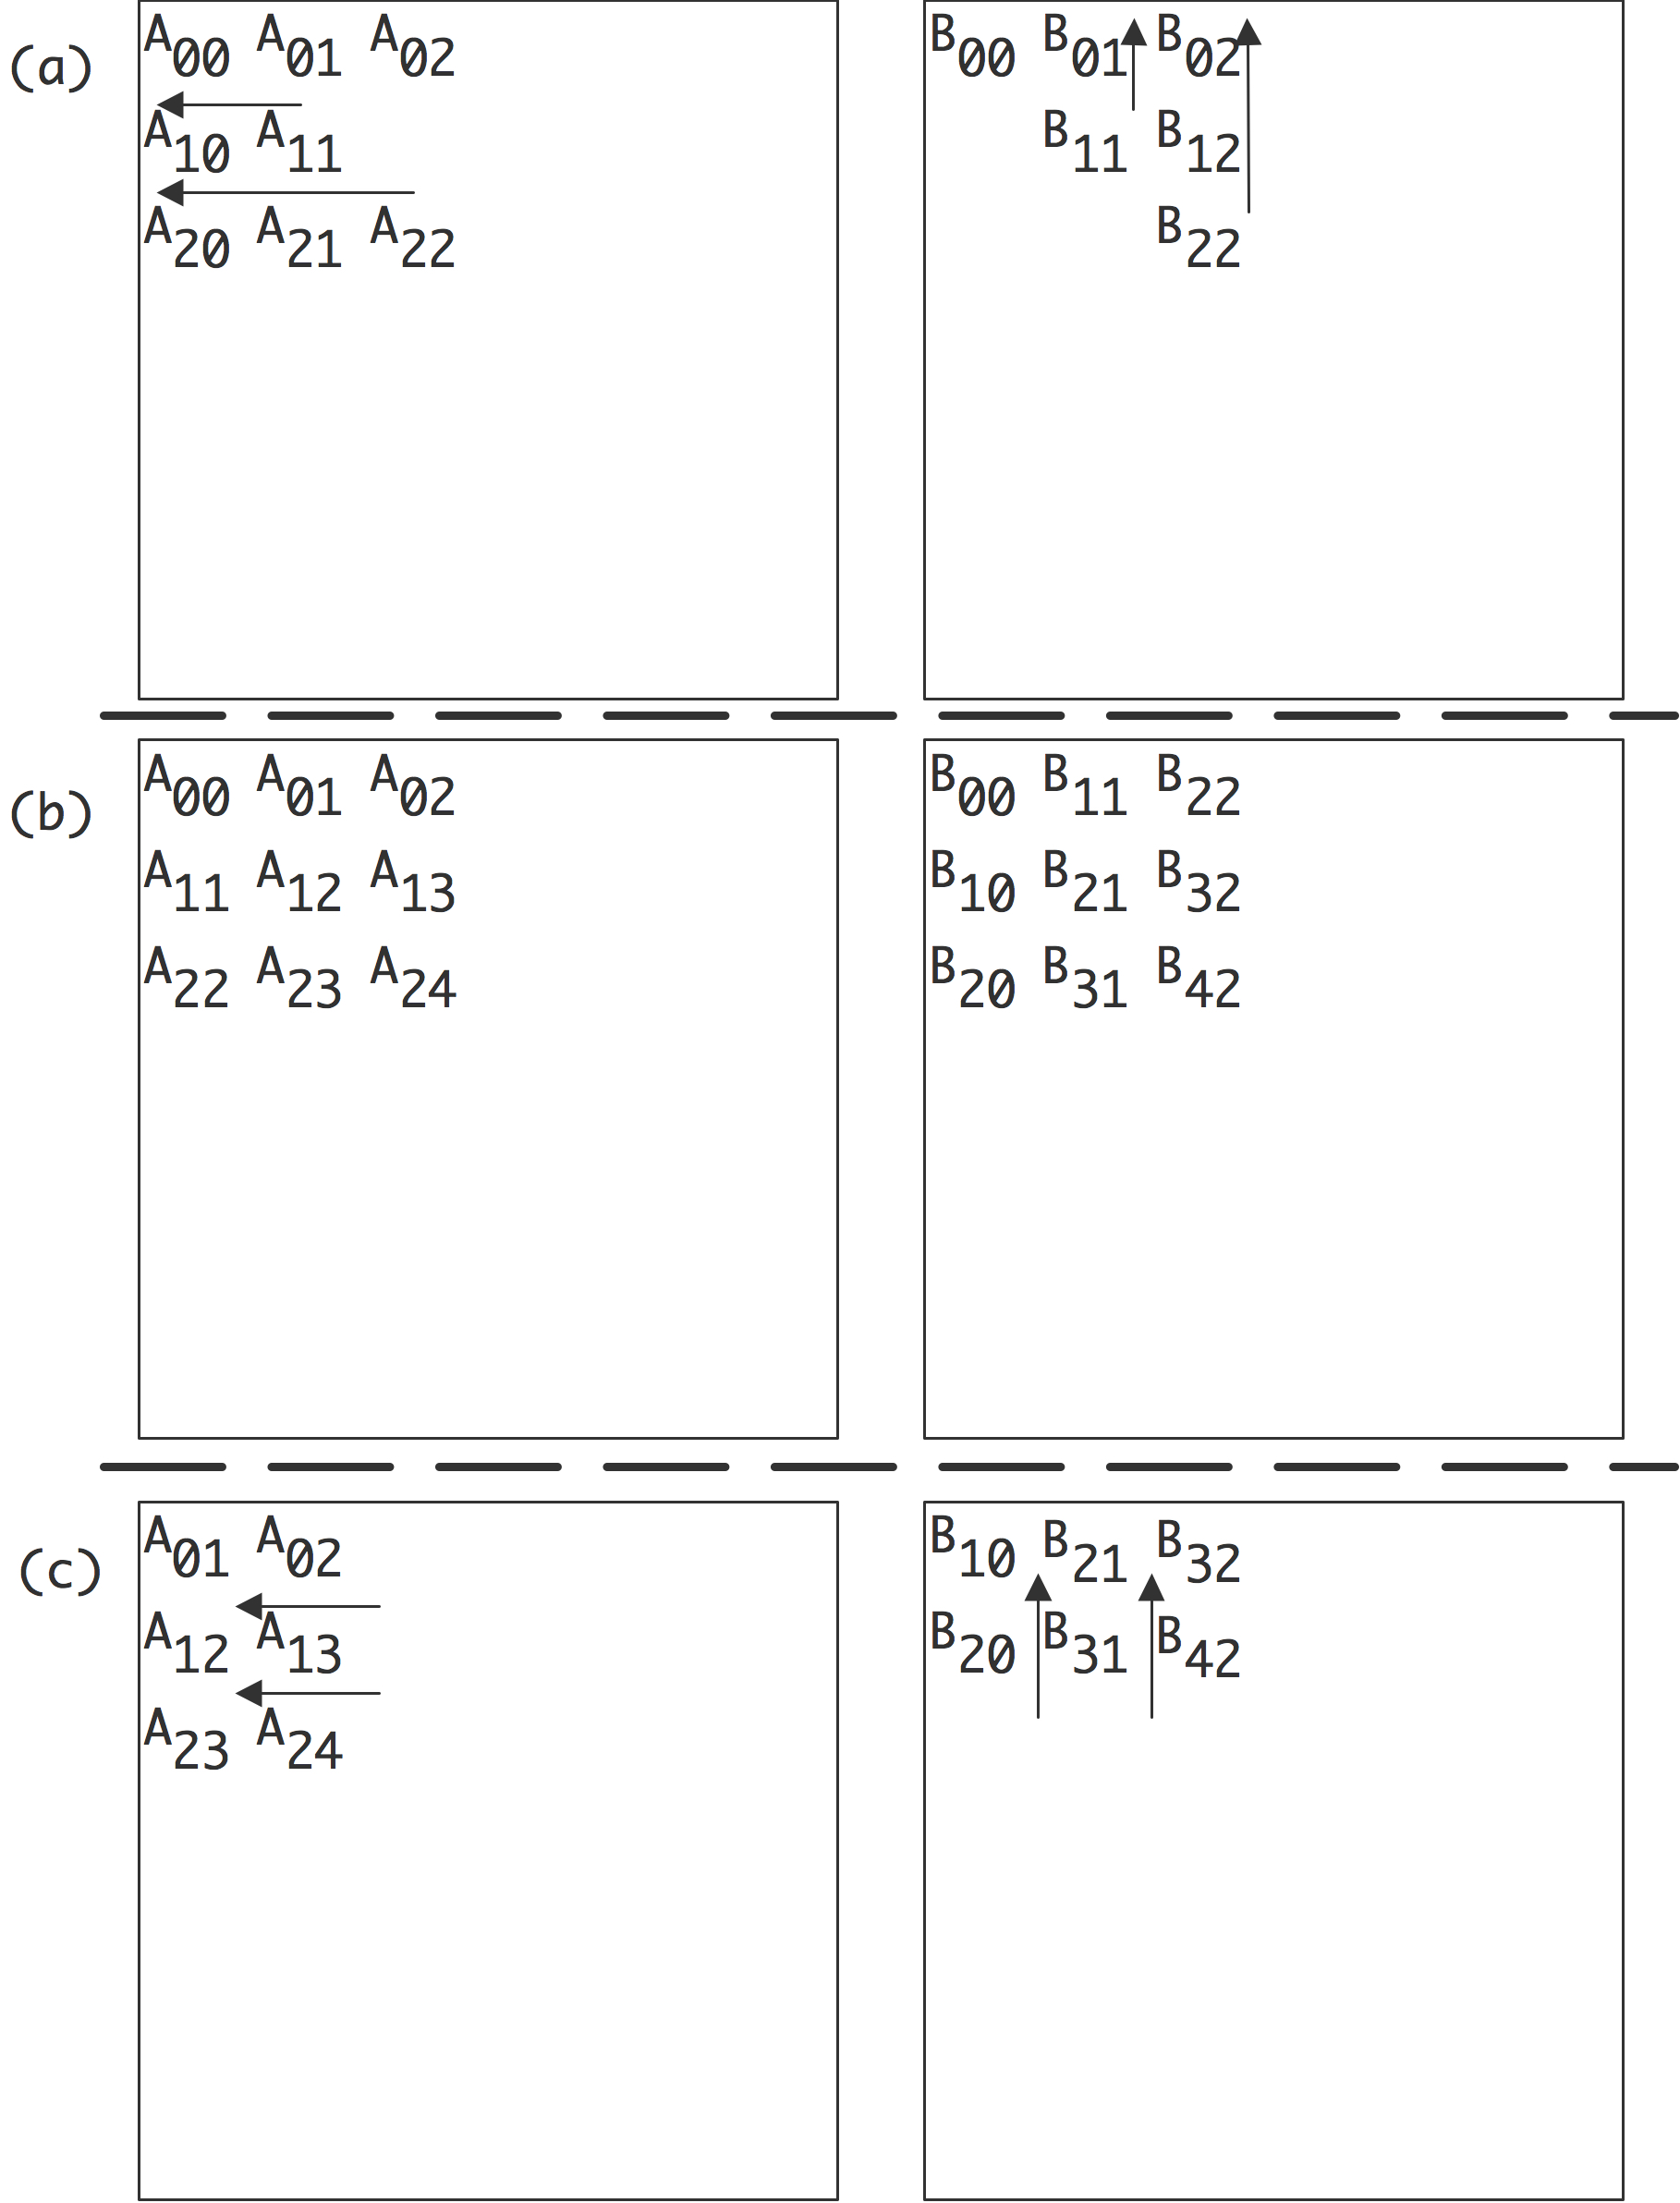
\includegraphics[scale=.15]{cannon1}
  \caption{Cannon's algorithm for matrix-matrix multiplication: (a) initial rotation of matrix rows and colums, (b)~resulting position in which processor~$(i,j)$ can start accumulating~$\sum_kA_{ik}B_{kj}$, (c)~subsequent rotation of $A,B$ for the next term.}
  \label{fig:cannon}
\end{wrapfigure}
%
One algorithm for this operation is known as
\emph{Cannon's algorithm}\index{matrix-matrix product!Cannon's algorithm for}.
It assumes a square processor grid where processor $(i,j)$ gradually
accumulates the $(i,j)$ block $C_{i,j}=\sum_kA_{i,k}B_{k,j}$;
see figure~\ref{fig:cannon}.

If you start top-left, you see that processor $(0,0)$ has both
$A_{00}$ and~$B_{00}$, so it can immediately start doing a local multiplication.
However, processor $(0,1)$ has $A_{01}$ and~$B_{01}$, which are
not needed together. However, if we rotate the second column of~$B$ up
by one position, processor~$(0,1)$ will have $A_{01},B_{11}$ and those
two do need to be multiplied. Similarly, we rotate the third column of~$B$
up by two places so that $(0,2)$ contains $A_{02},B_{22}$.

How does this story go in the second row? Processor~$(1,0)$ has
$A_{10},B_{10}$ which are not needed together. If we rotate
the second row of~$A$ one position to the left, it contains
$A_{11},B_{10}$ which are needed for a partial product.
And now processor~$(1,1)$ has $A_{11},B_{11}$.

If we continue this story, we start with a matrix~$A$ of which the
rows have been rotated left, and $B$ of which the columns have been rotated up.
In this setup, processor~$(i,j)$ contains $A_{i,i+j}$ and~$B_{i+j,j}$,
where the addition is done modulo the matrix size. This means that
each processor can start by doing a local product.

Now we observe that $C_{ij}=\sum_kA_{ik}B_{kj}$ implies that
the next partial product term comes from increasing~$k$ by~$1$.
The corresponding elements of $A,B$ can be moved into the processor
by rotating the rows and columns by another location.

\index{Dense linear algebra|)}

\Level 0 {Sparse matrix-vector product}
\label{sec:pspmvp}
\index{matrix-vector product!sparse|see{sparse, matrix-vector product}}

In linear system solving through iterative methods (see
section~\ref{sec:iterative}) the matrix-vector product is
computationally an important kernel, since it is executed in each of
potentially hundreds of iterations. In this section we look at
performance aspects of the matrix-vector product on a single
processor first; the multi-processor case will get our attention in
section~\ref{sec:pspmvp}.

\Level 1 {The single-processor sparse matrix-vector product}
\label{sec:spmvp-performance}

We are not much worried about the dense matrix-vector product in the
context of iterative methods, since one typically does not iterate on
dense matrices. In the case that we are dealing with block matrices,
refer to section~\ref{sec:mvp-opt} for an analysis of the dense
product. The sparse product is a lot trickier, since most of that
analysis does not apply.

\heading{Data reuse in the sparse matrix-vector product}

There are some similarities between the dense matrix-vector product,
executed by rows, and the \ac{CRS} sparse product
(section~\ref{sec:crs-mvp}). In both cases all matrix elements are
used sequentially, so any cache line loaded is utilized
fully. However, the \ac{CRS} product is worse at least the following
ways:
\begin{itemize}
\item The indirect addressing requires loading the elements of an
  integer vector. This implies that the sparse product has more memory
  traffic for the same number of operations.
\item The elements of the source vector are not loaded sequentially,
  in fact they can be loaded in effectively a random order. This means
  that a cacheline contains a source element will likely not be fully
  utilized. Also, the prefetch logic of the memory subsystem
  (section~\ref{sec:prefetch}) cannot assist here.
\end{itemize}
For these reasons, an application that is computationally dominated by
the sparse matrix-vector product can very well be run at $\approx5\%$
of the peak performance of the processor.

It may be possible to improve this performance if the structure of the
matrix is regular in some sense. One such case is where we are dealing
with a \indexterm{block matrix} consisting completely of small dense
blocks. This leads at least to a reduction in the amount of indexing
information: if the matrix consists of $2\times2$ blocks we get a
$4\times$ reduction in the amount of integer data transferred.
\begin{exercise}
  Give two more reasons why this strategy is likely to improve
  performance. Hint: cachelines, and reuse.
\end{exercise}
Such a \indextermbus{matrix}{tesselation} may give a factor of~2 in
performance improvement. Assuming such an improvement, we may adopt
this strategy even if the matrix is not a perfect block matrix: if
every $2\times2$ block will contain one zero element we may still get
a factor of~$1.5$ performance
improvement~\cite{vuduc:thesis,ButtEijkLang:spmvp}.

\heading{Vectorization in the sparse product}

In other circumstances bandwidth and reuse are not the dominant concerns:
\begin{itemize}
\item On old vector computers, such as old \indexterm{Cray} machines,
  memory was fast enough for the processor, but vectorization was
  paramount. This is a problem for sparse matrices, since the number
  of zeros in a matrix row, and therefore the vector length, is
  typically low.
\item On \acp{GPU} memory bandwidth is fairly high, but it is
  necessary to find large numbers of identical operations. Matrix can
  be treated independently, but since the rows are likely of unequal
  length this is not an appropriate source of parallelism.
\end{itemize}
For these reasons, a variation on the \indexterm{diagonal storage}
scheme for sparse matrices has seen a revival
recently. The observation here is that
if you sort the matrix rows by the number of rows you get a small
number of blocks of rows; each block will be fairly large, and in each
block the rows have the same number of elements.

A matrix with such a structure is good for vector
architectures~\cite{DAzevedo2005:vector-mvp}. In this case the product
is computed by diagonals.
\begin{exercise}
  Write pseudo-code for this case. How did the sorting of the rows
  improve the situation?
\end{exercise}

This sorted storage scheme also solves the problem we noted on
\acp{GPU}~\cite{Bolz:GPUsparse}. In this case we the traditional
\ac{CRS} product algorithm, and we have an amount of parallelism equal
to the number of rows in a block.

Of course there is the complication that we have permuted the matrix:
the input and output vectors will need to be permuted accordingly. If
the product operation is part of an iterative method, doing this
permutation back and forth in each iteration will probably negate any
performance gain. Instead we could permute the whole linear system and
iterate on the permuted system.
\begin{exercise}
  Can you think of reasons why this would work? Reasons why it wouldn't?
\end{exercise}

\Level 1 {The parallel sparse matrix-vector product}
\index{sparse!matrix-vector product!parallel|(}
\input chapters/spmvp
\index{sparse!matrix-vector product!parallel|)}

\begin{notready}
\Level 0 {Parallelism in solving linear systems from \acp{PDE}}

The numerical solution of \acp{PDE} is an important activity,
and the precision required often makes it a prime candidate for
parallel treatment. If we wonder just how parallel we can be,
and in particular what sort of a speedup is attainable,
we need to distinguish between various aspects of the question.

First of all we can ask if there is any intrinsic parallelism
in the problem. On a global level this will typically not be the case
(if parts of the problem were completely uncoupled, then they would be
separate problems, right?) but on a smaller level there may be
parallelism. 

For instance, looking at time-dependent problems, and referring to
section~\ref{sec:region-influence}, we can say that every next time
step is of course dependent on the previous one, but not every
individual point on the next time step is dependent on every point in
the previous step: there is a \indexterm{region of influence}. 
Thus it may be possible to partition the problem domain and
obtain parallelism.
\end{notready}


\Level 0 {Computational aspects of iterative methods}
\label{sec:iterative-computational}

All iterative methods feature the following operations:
\begin{itemize}
\item A matrix-vector product; this was discussed for the sequential
  case in section~\ref{sec:sparse} and for the parallel case in
  section~\ref{sec:pspmvp}.
  In the parallel case,
  construction of \ac{FEM} matrices has a complication that we will
  discuss in section~\ref{sec:fem-assembly}.
\item The construction of the preconditioner matrix~$K\approx A$, and
  the solution of systems $Kx=y$. This was discussed in the sequential
  case in section~\ref{sec:preconditioner}. Below
  we will go into parallelism aspects in section~\ref{sec:parallel-prec}.
\item Some vector operations (including inner products, in
  general). These will be discussed next.
\end{itemize}

\Level 1 {Vector operations}

There are two types of vector operations in a typical iterative method:
vector additions and inner products. 

\begin{exercise}
  Consider the \ac{CG} method of section~\ref{sec:cg},
  figure~\ref{fig:pcg}, applied to the
  matrix from a 2D \ac{BVP}; equation~\eqref{eq:5starmatrix}, First
  consider the unpreconditioned case $M=I$. Show that there is a
  roughly equal number of floating point
  operations are performed in the matrix-vector product and 
  in the vector operations. Express everything in the matrix size~$N$ and
  ignore lower order terms. How would this balance be if the matrix
  had 20 nonzeros per row?

  Next, investigate this balance between vector and matrix operations
  for the \ac{FOM} scheme in section~\ref{sec:fom}. Since the number
  of vector operations depends on the iteration, consider the first 50
  iterations and count how many floating point operations are done in
  the vector updates and inner product versus the matrix-vector
  product. How many nonzeros does the matrix need to have for these
  quantities to be equal?
\end{exercise}

\begin{exercise}
  Flop counting is not the whole truth. What can you say about the
  efficiency of the vector and matrix operations in an iterative
  method, executed on a single processor?
\end{exercise}

\Level 2 {Vector additions}

The vector additions are
typically of the form $x\leftarrow x+\alpha y$ or $x\leftarrow \alpha x+y$.
If we assume that all vectors are distributed the same way, this
operation is fully parallel.

\Level 2 {Inner products}
\index{inner products|(}

Inner products are vector operations, but they are computationally
more interesting than updates, since they involve communication. 

When we compute an inner product, most likely 
every processor needs to receive the computed value. We
use the following algorithm:

\begin{displayalgorithm}
  \For {processor $p$} {
    compute $a_p\leftarrow x_p^ty_p$ where $x_p,y_p$ are the part of
    $x,y$ stored on processor~$p$ }
    do a global reduction to compute $a=\sum_p a_p$ \;
    broadcast the result
  \caption{Compute $a\leftarrow x^ty$ where $x,y$ are distributed vectors}
\end{displayalgorithm}

The reduction and broadcast (which can be joined into an {\tt
  Allreduce}) combine data over all processors, so they have a
communication time that increases with the number of processors. This
makes the inner product potentially an expensive operation, and people
have suggested a number of ways to reducing their impact on the
performance of iterative methods.

\begin{exercise}
  Iterative methods are typically used for sparse matrices. In that
  context, you can argue that the communication involved in an inner product
  can have a larger influence on overall performance than the
  communication in the matrix-vector product. What is the
  complexity of the matrix-vector product and the inner product as a
  function of the number of processors?
\end{exercise}

Here are some of the approaches that have been taken.
\begin{itemize}
\item The \ac{CG} method has two inner products per iteration that are
  inter-dependent. It is possible to rewrite the method so that it
  computes the same iterates (in exact arithmetic, at least) but so
  that the two inner products per iteration can be
  combined. See~\cite{ChGe:sstep,DAzEijRo:ppscicomp,Me:multicg,YandBrent:bicgstab}.
\item It may be possible to overlap the inner product calculation with
  other, parallel, calculations~\cite{dehevo92:acta}.
\item In the \ac{GMRES} method, use of the classical \acf{GS}
  method takes far fewer independent inner product than the modified
  \ac{GS} method, but it is less stable. People have investigated strategies for deciding
  when it is allowed to use the classic \ac{GS} method~\cite{Langou:thesis}.
\end{itemize}

Since computer arithmetic is not associative, inner products are a prime
source of results that differ when the same calculation is executed of
two different processor configurations. In section~\ref{sec:roundoff-parallel}
we sketched a solution.

\index{inner products|)}

\Level 1 {Finite element matrix construction}
\label{sec:fem-assembly}

The \indexac{FEM} leads to an interesting issue in parallel
computing. For this we need to sketch the basic outline of how this
method works. The \ac{FEM} derives its name from the fact that the
physical objects modeled are divided into small two or three
dimensional shapes, the elements, such as triangles and squares in 2D,
or pyramids and bricks in~3D. On each of these, the function we are
modeling is then assumed to polynomial, often of a low degree, such as
linear or bilinear.

\begin{figure}[ht]
  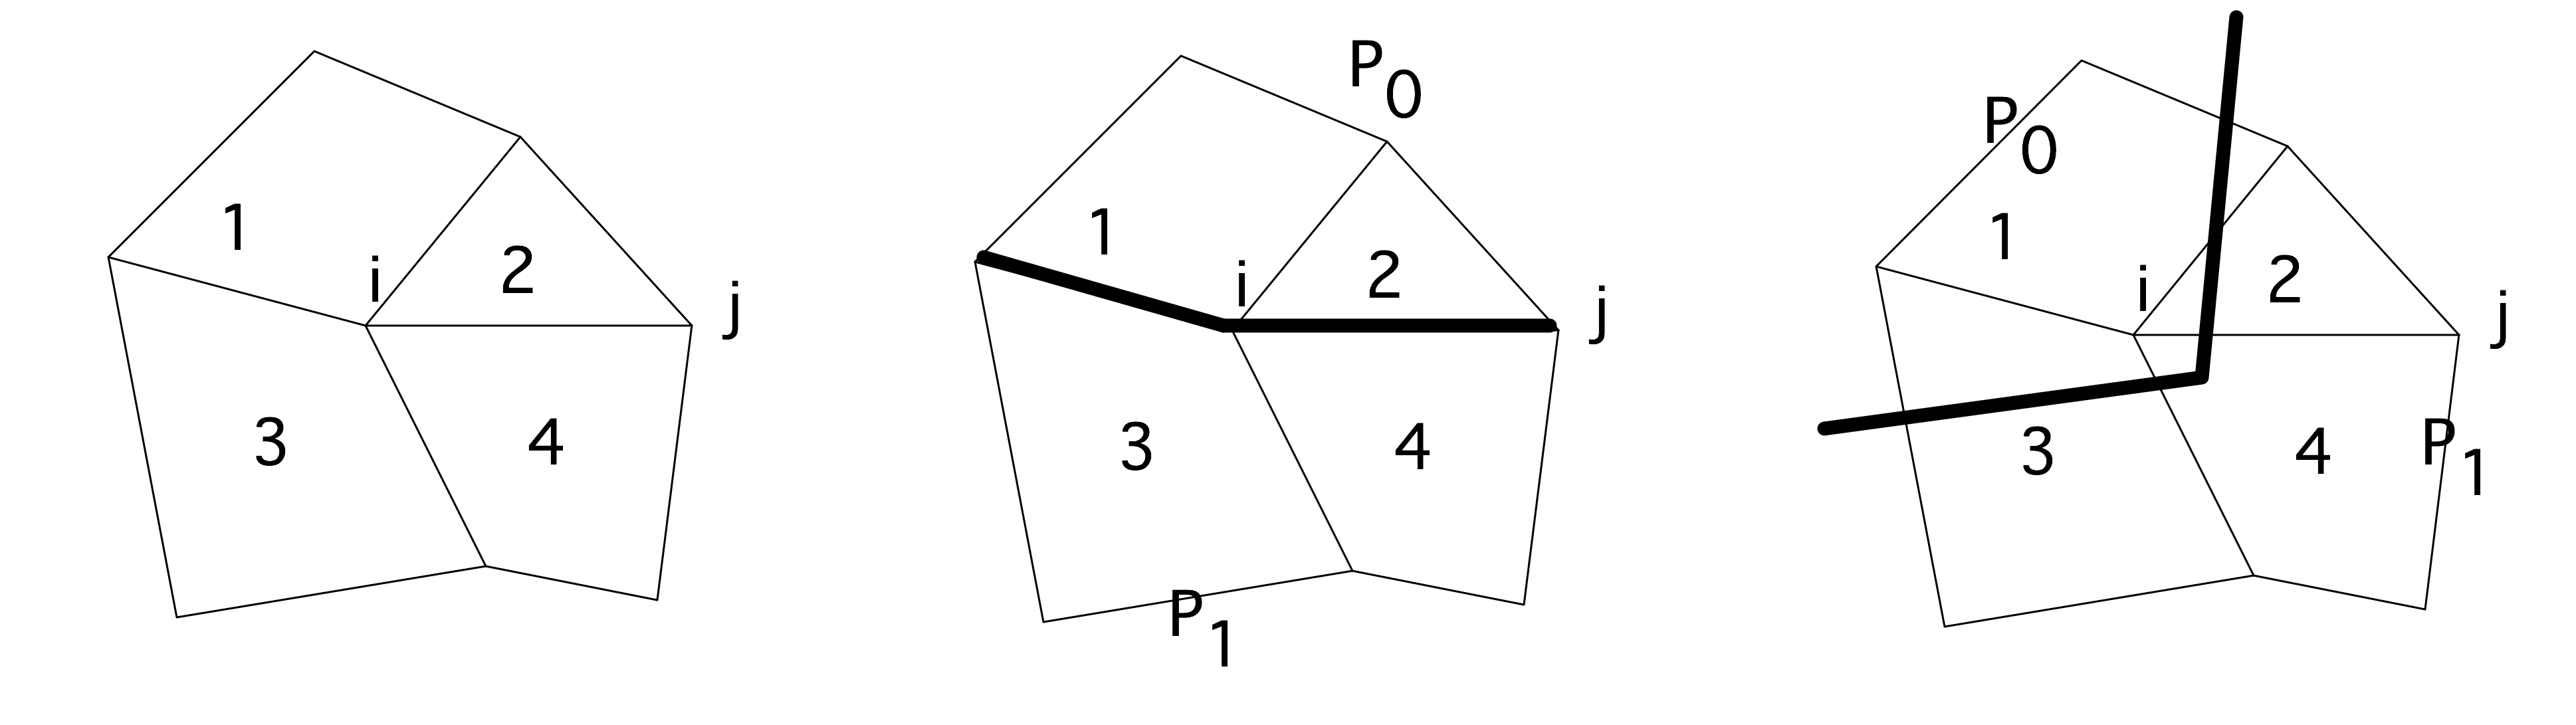
\includegraphics[scale=.12]{graphics/fem}  
  \caption{A finite element domain, parallelization of the matrix
    construction, and parallelization of matrix element storage}
  \label{fig:fem-assembly}
\end{figure}

The crucial fact is that a matrix element~$a_{ij}$ is then the sum of
computations, specifically certain integrals, over all elements that
contain both variables $i$ and~$j$:
\[ a_{ij}=\sum_{e\colon i,j\in e} a^{(e)}_{ij}. \]
The computations in each element share many common parts, so it is
natural to assign each element~$e$ uniquely to a processor~$P_e$,
which then computes all contributions~$a^{(e)}_{ij}$. In
figure~\ref{fig:fem-assembly} element~2 is assigned to processor~0
and element~4 to processor~1.

Now consider variables $i$ and~$j$ and the matrix
element~$a_{ij}$.  It is constructed as the sum of computations over
domain elements 2 and~4, which have been assigned to different processors.
Therefore, no matter what processor row $i$ is assigned to, at least
one processor will have to communicate its contribution to matrix
element~$a_{ij}$.

Clearly it is not possibly to make assignments $P_e$ of elements and
$P_i$ of variables such that $P_e$ computes in full the coefficients
$a_{ij}$ for all $i\in e$. In other words, if we compute the
contributions locally, there needs to be some amount of communication to
assemble certain matrix elements.
For this reason, modern linear algebra libraries such as PETSc (see
tutorial section~\ref{tut:petsc}) allow any processor to set any
matrix element.

\Level 1 {A simple model for iterative method performance}

Above, we have already remarked that iterative methods have very little
opportunity for data reuse, and they are therefore characterized as
\indexterm{bandwidth-bound} algorithms. This allows us to make a simple
prediction as to the \indextermsub{floating point performance of}{iterative methods}.
Since the number of iterations of an iterative method is hard to predict,
by performance here we mean the performance of a single iteration.
Unlike with \indextermbus{direct methods}{for linear systems}
(see for instance section~\ref{sec:dissection}),
the number of flops to solution is very hard to establish in advance.

First we argue that we can restrict ourselves to the \emph{performance of the sparse
  matrix vector product}\index{sparse!matrix-vector product!performance of}:
the time spent in this operation is considerably more than in the vector operations.
Additionally, most preconditioners have a computational structure that is
quite similar to the matrix-vector product.

Let us then consider the \emph{performance of the CRS matrix-vector
  product}\index{Compressed Row Storage (CRS)!performance of the
  matrix-vector product}.
\begin{itemize}
\item First we observe that the arrays of matrix elements and column indices have no reuse,
  so the performance of loading them is completely determined by the available bandwidth.
  Caches and prefect streams only hide the latency, but do not improve the bandwidth.
  For
  each multiplication of matrix element times input vector element
  we load one floating point number and one integer. Depending one whether the
  indices are 32-bit or 64-bit, this means 12 or 16~bytes loaded for each multiplication.
\item The demands for storing the result vector are less important: an output vector
  element is written only once for each matrix row.
\item The input vector can also be ignored in the bandwidth calculation.
  At first sight you might think that indirect indexing
  into the input vector is more or less random and therefore expensive.
  However, let's take the operator view of a matrix-vector product
  and consider the space domain of the \ac{PDE} from which the matrix stems;
  see section~\ref{sec:2dbvp}. We now see that the seemingly random indexing
  is in fact into vector elements that are grouped closely together.
  This means that these vector elements will likely reside in L3 cache,
  and therefore accessible with a higher bandwidth (say, by a factor of at least~5)
  than data from main memory.
\end{itemize}
For the parallel performance of the sparse matrix-vector product we
consider that in a \ac{PDE} context each processor communicates only
with a few neighbours. Furthermore, a surface-to-volume argument
shows that the message volume is of a lower order than the on-node
computation.

In sum, we conclude that a very simple model for the sparse matrix vector product,
and thereby for the whole iterative solver, consists of measuring
the effective bandwidth and computing the performance as one
addition and one multiplication operation per 12 or 16~bytes loaded.

\Level 0 {Parallel preconditioners}
\label{sec:parallel-prec}

Above (section~\ref{sec:preconditioner} and in particular~\ref{sec:ilu}) we saw a
couple of different choices of~$K$. In this section we will begin the
discussion of parallelization strategies. The discussion is continued
in detail in the next sections.

\Level 1 {Jacobi preconditioning}

The Jacobi method (section~\ref{sec:jacobi-seidel}) uses the diagonal
of~$A$ as preconditioner. Applying this is as parallel as is
possible: the statement $y\leftarrow K\inv x$ scales every element of
the input vector independently. Unfortunately the improvement in the
number of iterations with a Jacobi preconditioner is rather
limited. Therefore we need to consider more sophisticated methods such
\ac{ILU}. Unlike with the Jacobi preconditioner, parallelism is then
not trivial.

\Level 1 {The trouble with parallel ILU}

Above we saw that, in a flop counting sense, applying an ILU
preconditioner (section~\ref{sec:ilu}) is about as expensive as doing
a matrix-vector product. This is no longer true if we run our
iterative methods on a parallel computer.

At first glance the operations are similar. A matrix-vector product
$y=Ax$ looks like
\begin{verbatim}
for i=1..n
  y[i] = sum over j=1..n a[i,j]*x[j]
\end{verbatim}
In parallel this would look like
\begin{verbatim}
for i=myfirstrow..mylastrow
  y[i] = sum over j=1..n a[i,j]*x[j]
\end{verbatim}
Suppose that a processor has local copies of all the elements of $A$
and~$x$ that it will need, then this operation is fully parallel: each
processor can immediately start working, and if the work load is
roughly equal, they will all finish at the same time. The total time
for the matrix-vector product is then divided by the number of
processors, making the speedup more or less perfect.

Consider now the forward solve $Lx=y$, for instance in the context of
an \ac{ILU} preconditioner:
\begin{verbatim}
for i=1..n
  x[i] = (y[i] - sum over j=1..i-1 ell[i,j]*x[j]) / a[i,i]
\end{verbatim}
We can simply write the parallel code:
\begin{verbatim}
for i=myfirstrow..mylastrow
  x[i] = (y[i] - sum over j=1..i-1 ell[i,j]*x[j]) / a[i,i]
\end{verbatim}
but now there is a problem. We can no longer say `suppose a processor
has local copies of everything in the right hand side', since the
vector~$x$ appears both in the left and right hand side. While the
matrix-vector product is in principle fully parallel over the matrix
rows, this triangular solve code is recursive, hence sequential.

In a parallel computing context this means that, for the second
processor to start, it needs to wait for certain components of~$x$
that the first processor computes. Apparently, the second processor
can not start until the first one is finished, the third processor has
to wait for the second, and so on. The disappointing conclusion is
that in parallel only one processor will be active at any time, and
the total time is the same as for the sequential algorithm. This is
actually not a big problem in the dense matrix case, since parallelism
can be found in the operations for handling a single row (see
section~\ref{sec:multicore-block}), but in the sparse case it means we
can not use incomplete factorizations without some redesign.

In the next few subsections we will see different strategies for
finding preconditioners that perform efficiently in parallel.

\Level 1 {Block Jacobi methods}
\label{sec:block-jacobi}
\index{block Jacobi|(}

Various approaches have been suggested to remedy this sequentiality
the triangular solve. For instance, we could simply let the processors
ignore the components of~$x$ that should come from other processors:
\begin{verbatim}
for i=myfirstrow..mylastrow
  x[i] = (y[i] - sum over j=myfirstrow..i-1 ell[i,j]*x[j]) 
         / a[i,i]
\end{verbatim}
This is not mathematically equivalent to the sequential algorithm
(technically, it is called a \indexterm{block Jacobi} method with 
\ac{ILU} as the \indexterm{local solve}), but
since we're only looking for an approximationg $K\approx A$, this is
simply a slightly cruder approximation.
\begin{exercise}
  Take the Gauss-Seidel code you wrote above, and simulate a parallel
  run. What is the effect of increasing the (simulated) number of processors?
\end{exercise}

The idea behind block methods can easily be appreciated pictorially;
see figure~\ref{fig:block-method}.
\begin{figure}[ht]
  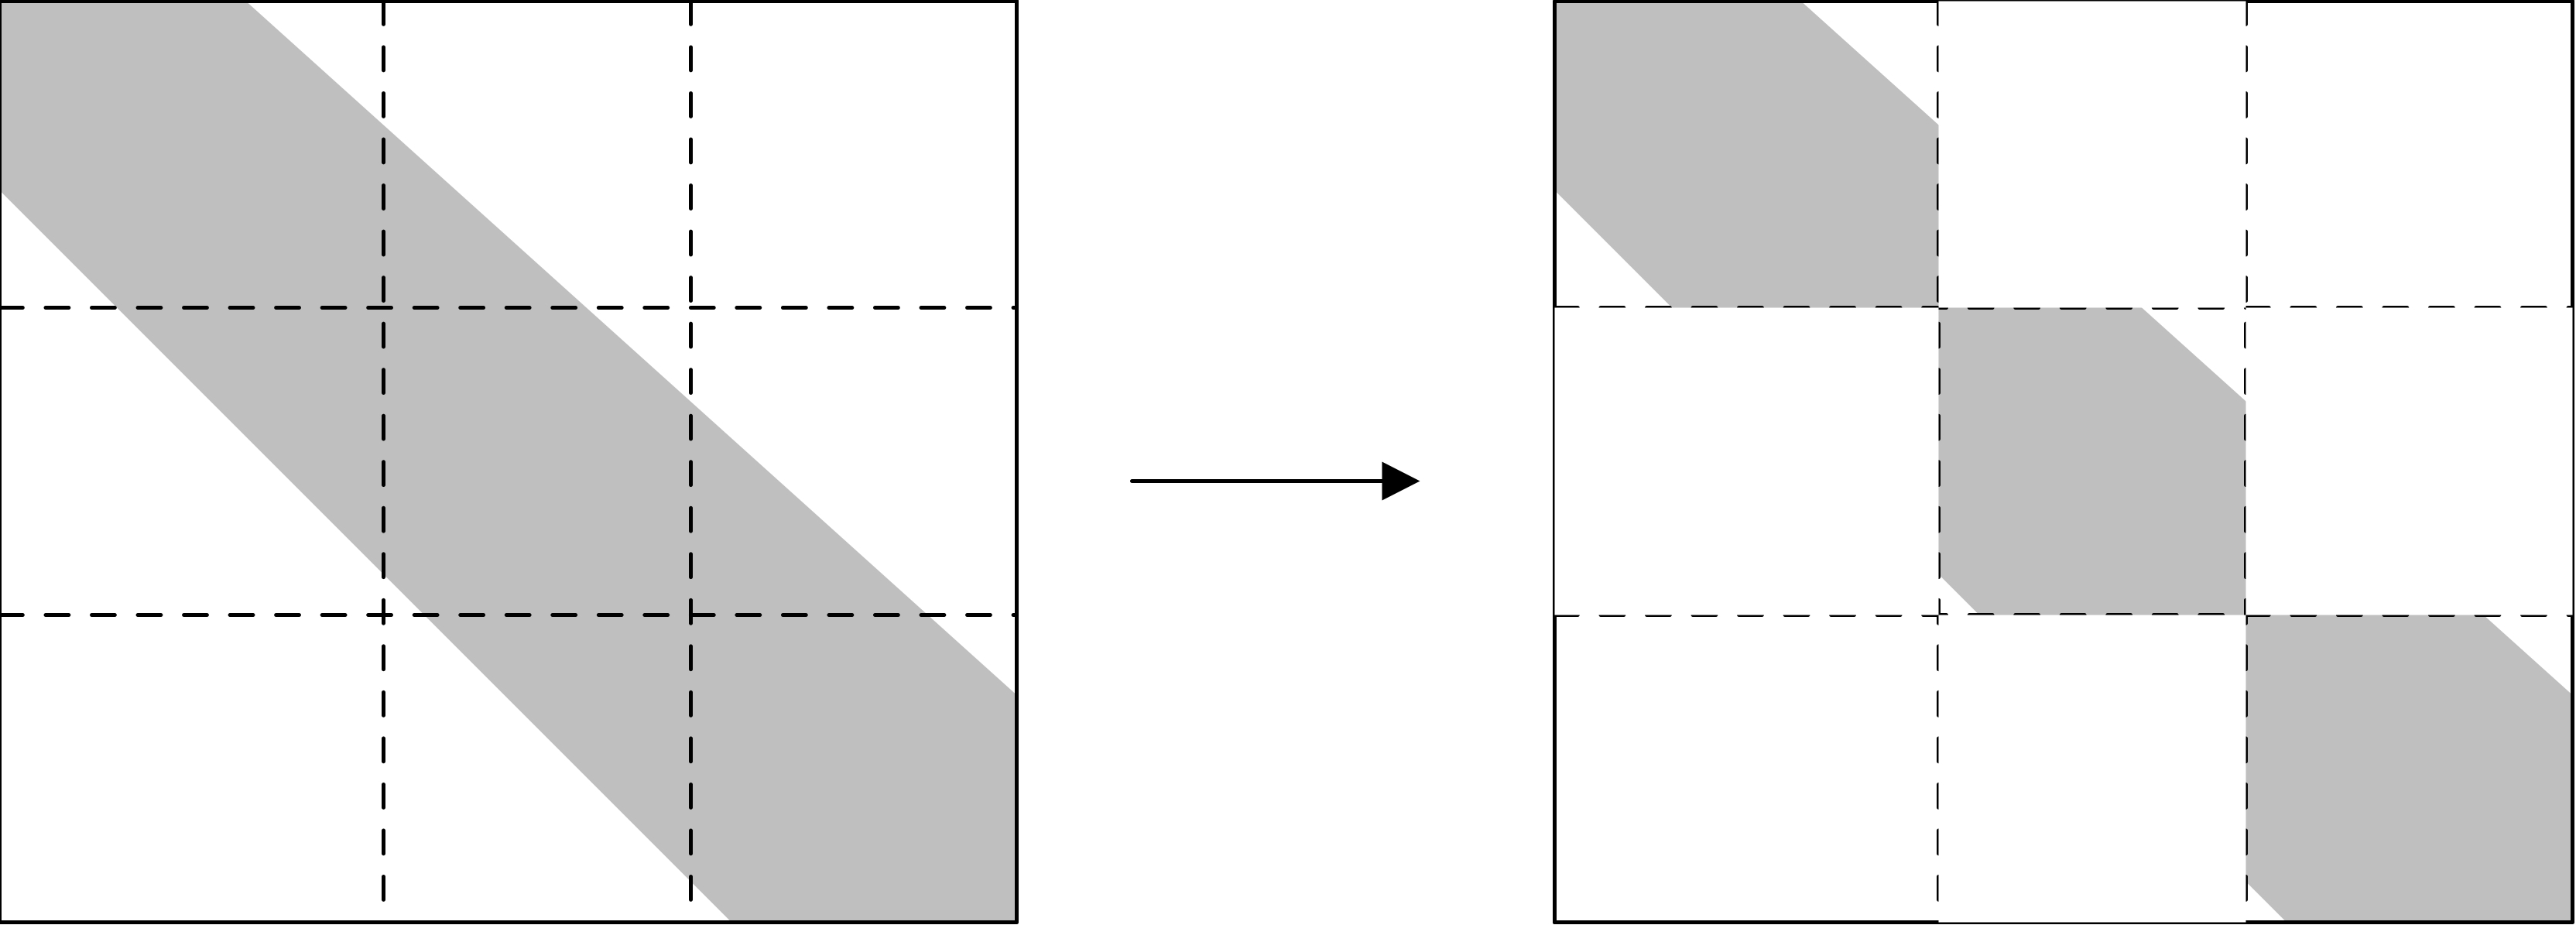
\includegraphics[scale=.12]{graphics/block-jacobi}
  \caption{Sparsity pattern corresponding to a block Jacobi
    preconditioner}
  \label{fig:block-method}
\end{figure}
In effect, we make an \ac{ILU} of the matrix that we get by ignoring
all connections between processors. Since in a \ac{BVP} all points
influence each other (see section~\ref{sec:region-influence}), using a
less connected preconditioner will increase the number of iterations
if executed on a sequential computer. However, block methods are
parallel and, as we observed above, a sequential preconditioner is
very inefficient in a parallel context, so we put up with this
increase in iterations.

\index{block Jacobi|)}

\Level 1 {Parallel ILU}
\label{sec:parallel-ilu}
\index{Incomplete LU (ILU)!parallel|(}

The Block Jacobi preconditioner operates by decoupling domain
parts. While this may give a method that is highly parallel, it may
give a higher number of iterations than a true \ac{ILU}
preconditioner. (A~theoretical argument can be made that this
decoupling decreases the efficiency of the iterative method; see
section~\ref{sec:region-influence}.) Fortunately it is possible to
have a parallel \ac{ILU} method.

In section~\ref{sec:redblackgreen} you saw the combination of
\indextermbus{graph}{colouring} and permutation. Let $P$ be the
permutation that groups like-coloured variables together, then $\tilde
A=P^tAP$ is a matrix with the following structure:
\begin{itemize}
\item $\tilde A$ has a block structure with the number of blocks equal
  to the number of colours in the adjacency graph of~$A$; and
\item each diagonal block is a diagonal matrix.
\end{itemize}
Now, if you are performing an iterative system solution
and you are looking for a parallel preconitioner you can use this
permuted matrix. Consider solving $Ly=x$ with the permuted system. We
write the usual algorithm (section~\ref{sec:lu-solve}) as
\begin{quotation}
  \begin{tabbing}
    for \=$c$ in the set of colours:\\
    \>for \=$i$ in the variables of colour $c$:\\
    \>\>$y_i\leftarrow x_i-\sum_{j<i} \ell_{ij}y_j$
  \end{tabbing}
\end{quotation}

\begin{exercise}
  Show that the flop count of solving a system $LUx=y$ remains the
  same (in the highest order term) when you from an \ac{ILU}
  factorization in the natural ordering to one in the colour-permuted
  ordering.
\end{exercise}

\begin{figure}
  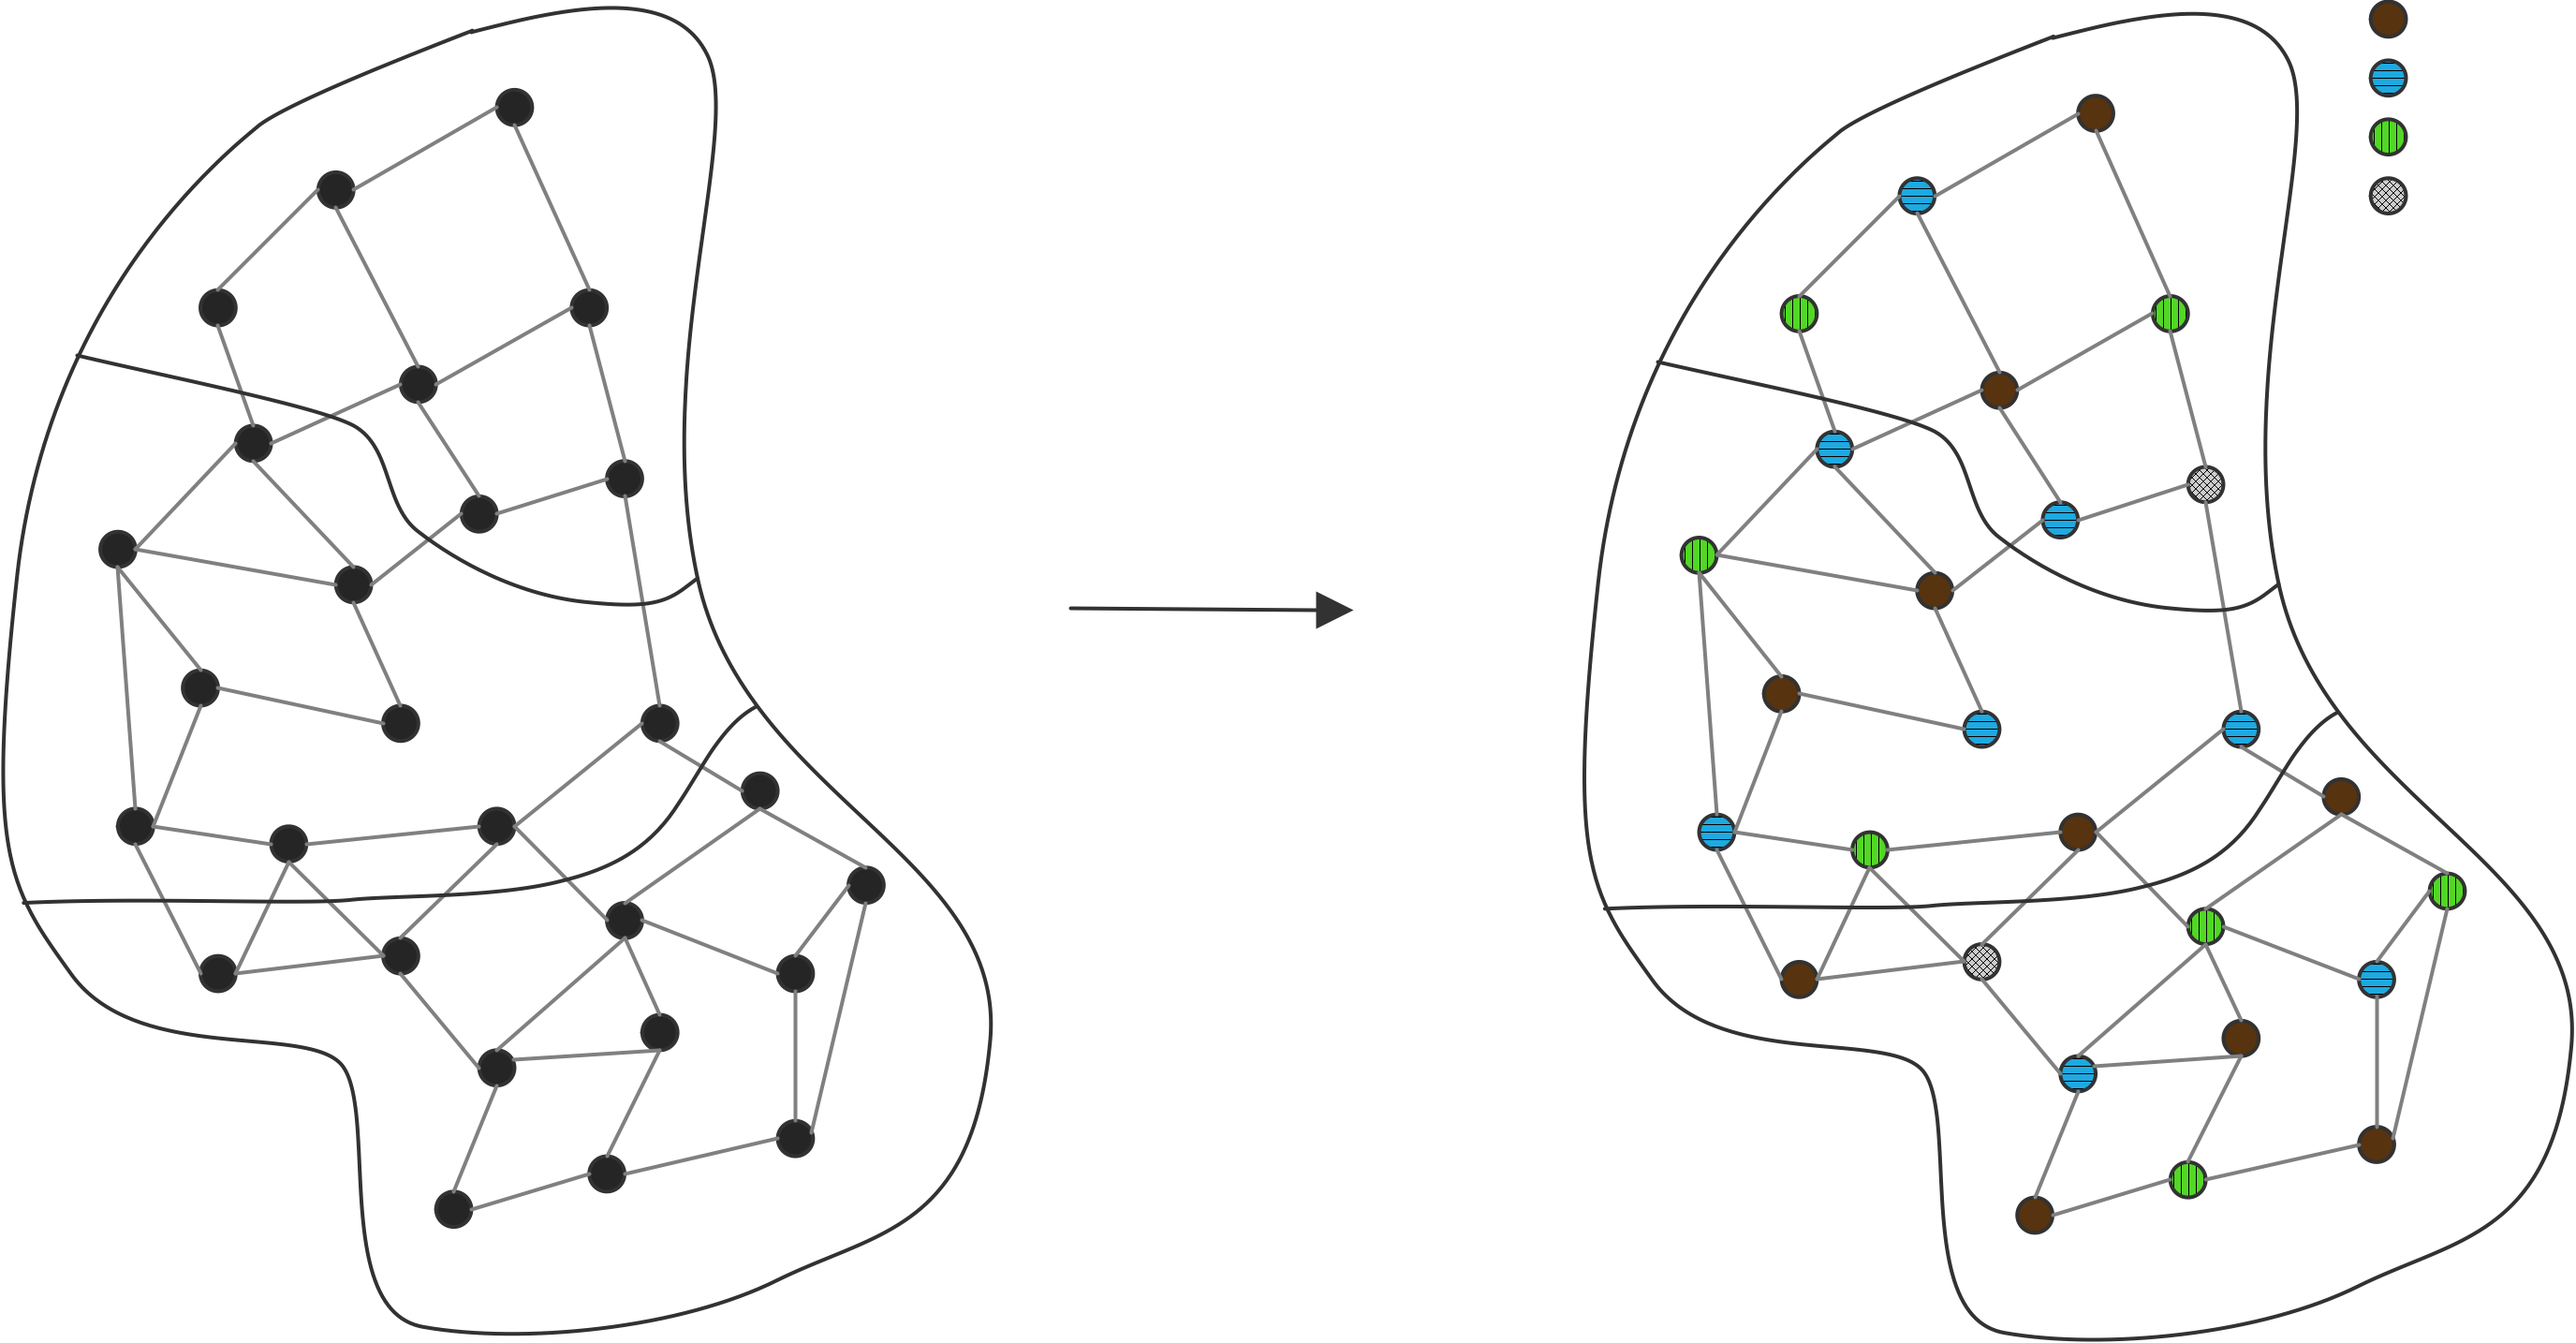
\includegraphics[scale=.12]{graphics/pilu}
  \caption{A partitioned domain with coloured nodes}
  \label{fig:pilu}
\end{figure}
Where does all this colouring get us? Solving is still
sequential\ldots Well, it is true that the outer loop over the colours
is sequential, but all the points of one colour are independent of
each other, so they can be solved at the same time.
\begin{figure}
  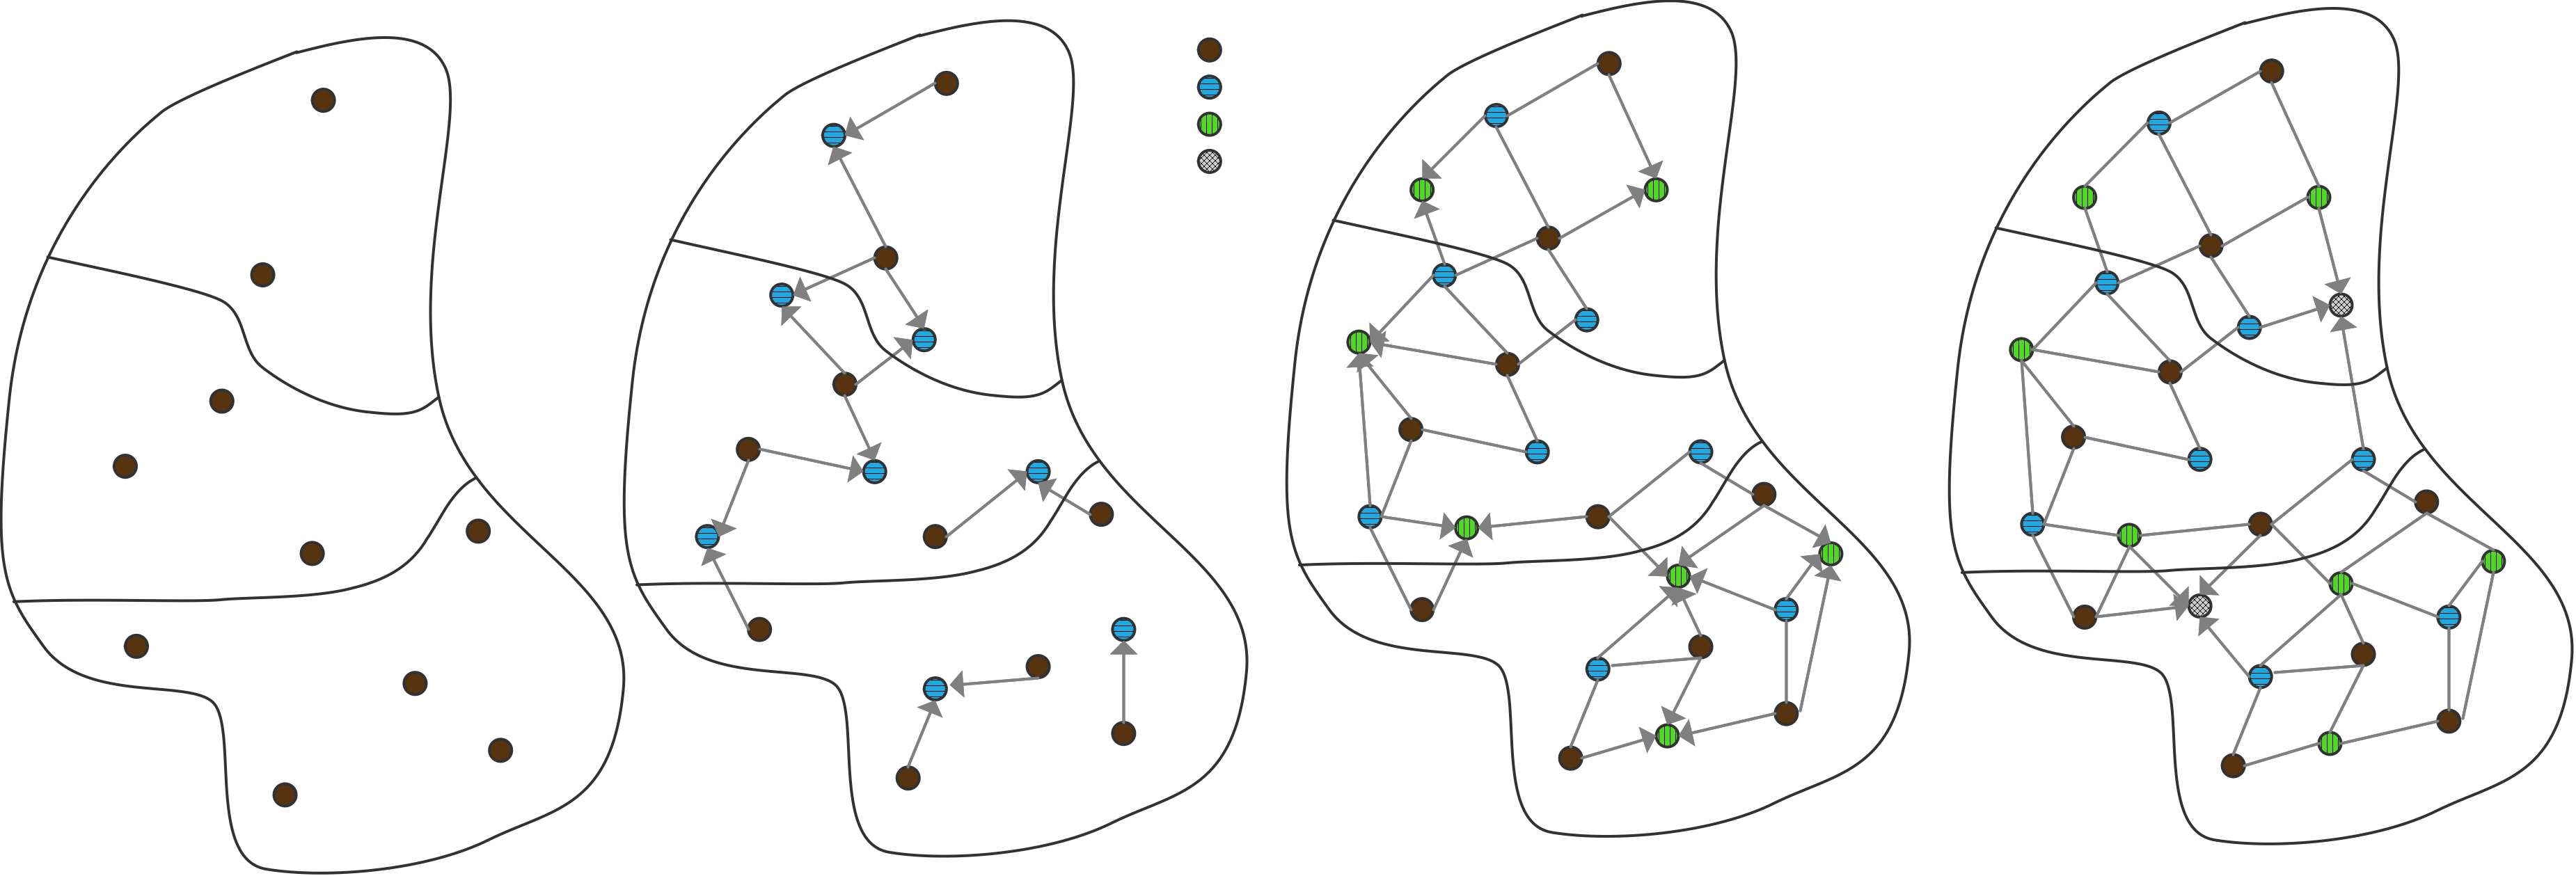
\includegraphics[scale=.13]{graphics/pilu-solve}
  \caption{Solving a parallel multicolour ILU in four steps}
  \label{fig:pilu-solve}
\end{figure}
So if we use an ordinary domain partitioning and combine that with a
multi-colouring (see figure~\ref{fig:pilu}), the processors are all
active during all the colour stages; see
figure~\ref{fig:pilu-solve}. Ok, if you take a close look at that
figure you'll see that one processor is not active in the last
colour. With large numbers of nodes per processor this is unlikely to
happen, but there may be some load inbalance.

\index{Incomplete LU (ILU)!parallel|)}

\Level 0 {Ordering strategies and parallelism}
\label{sec:ordering}

In the foregoing we have remarked on the fact that solving
a linear system of equations is inherently a recursive activity.
For dense systems, the number of operations is large enough
compared to the recursion length that finding parallelism 
is fairly straightforward. Sparse systems, on the other hand,
take more sophistication. In this section we will look at 
a number of strategies for reordering the equations (or, equivalently,
permuting the matrix) that will increase the available parallelism.

These strategies can all be considered as variants of Gaussian elimination.
By making incomplete variants of them (see section~\ref{sec:ilu}),
all these strategies also apply to constructing preconditioners
for iterative solution methods.

\Level 1 {Nested dissection}
\label{sec:dissection}
\index{nested dissection|(}
\input chapters/dissection
\index{nested dissection|)}
\Level 1 {Variable reordering and colouring: independent sets}
\label{sec:redblackgreen}
\input chapters/redblackgreen

\Level 0 {Operator splitting}

In some contexts, it is necessary to perform implicit calculations
through all directions of a two or three-dimensional array. For
example, in section~\ref{sec:heateq} you saw how the implicit solution
of the heat equation
gave rise to repeated systems
\begin{equation}
  (\alpha I+\frac {d^2}{dx^2}+\frac{d^2}{dy^2})u^{(t+1)}=u^{(t)}
  \label{eq:heat-recap}
\end{equation}
Without proof, we state that the time-dependent problem can also be solved by
\begin{equation}
  (\beta I+\frac {d^2}{dx^2})(\beta I+\frac{d^2}{dy^2})u^{(t+1)}=u^{(t)}
  \label{eq:adi-recap}
\end{equation}
for suitable~$\beta$. This scheme will not compute the same
values on each individual time step, but it will converge to the same
steady state. The scheme can also be used as a preconditioner in the
\ac{BVP} case.

This approach has considerable advantages, mostly in terms of
operation counts: the original system has to be solved either making a
factorization of the matrix, which incurs \indexterm{fill-in}, or by
solving it iteratively.

\begin{exercise}
  Analyze the relative merits of these approaches, giving rough
  operation counts. Consider both the case where $\alpha$ has
  dependence on~$t$ and where it does not. Also discuss the expected
  speed of various operations.
\end{exercise}

A further advantage appears when we consider the parallel solution
of~\eqref{eq:adi-recap}. Note that we have a two-dimensional set of
variables~$u_{ij}$, but the operator $I+d^2u/dx^2$ only connects
$u_{ij},u_{ij-1},u_{ij+1}$. That is, each line corresponding to an
$i$~value can be processed independently. Thus, both operators can be
solved fully parallel using a one-dimensional partition on the domain.
The solution of a the system in~\eqref{eq:heat-recap}, on the other
hand, has limited parallelism.

Unfortunately, there is a serious complication: the operator in $x$
direction needs a partitioning of the domain in on direction, and the
operator in $y$ in the other. The solution usually taken is to
transpose the $u_{ij}$ value matrix in between the two solves, so that
the same processor decomposition can handle both. This transposition
can take a substantial amount of the processing time of each time step.

\begin{exercise}
  Discuss the merits of and problems with a two-dimensional
  decomposition of the domain, using a grid of $P=p\times p$
  processors. Can you suggest a way to ameliorate the problems?
\end{exercise}

One way to speed up these calculations, is to replace the implicit
solve, by an explicit operation; see
section~\ref{sec:implicit-becomes-explicit}.

\Level 0 {Parallelism and implicit operations}
\label{sec:parallel-implicit}
\input chapters/implicit

\Level 0 {Grid updates}

One of the conclusions of chapter~\ref{ch:odepde} was that explicit
methods for time-dependent problems are computationally easier than
implicit ones.  For instance, they typically involve a matrix-vector
product rather than a system solution, and parallelizing explicit
operations is fairly simple: each result value of the matrix-vector
product can be computed independently. That does not mean that there
are other computational aspects worth remarking on.

Since we are dealing with sparse matrices, stemming from some computational stencil,
we take the operator point of view. In figures \ref{fig:laplaceparallel} 
and~\ref{fig:ghost} you saw how applying a stencil in each point of the domain 
induces certain relations between processors: in order to evaluate the matrix-vector
product $y\leftarrow Ax$ on a processor, that processor needs to obtain the $x$-values
of its \indexterm{ghost region}. Under reasonable assumptions on the partitioning
of the domain over the processors, the number of messages involved will be fairly
small.

\begin{exercise}
Reason that, in a \ac{FEM} or \ac{FDM} context,
the number of messages is $O(1)$ as~$h\downarrow\nobreak 0$.
\end{exercise}

In section~\ref{sec:reuse} you saw that the matrix-vector product has
little data reuse, though there is some locality to the computation;
in section~\ref{sec:crs-mvp} it was pointed out that the locality of the 
sparse matrix-vector product is even worse because of
indexing schemes that the sparsity necessitates. This means that the sparse
product is largely a \emph{bandwidth-bound algorithm}. 

Looking at just a
single product there is not much we can do about that. 
However, 
often we do a number of such products in a row, for instance as the steps
in a time-dependent process. In that case there may be rearrangements
of the operations that lessen the bandwidth demands. Consider as a simple example
\begin{equation}
\forall_i\colon x^{(n+1)}_i = f\bigl( x^{(n)}_i, x^{(n)}_{i-1}, x^{(n)}_{i+1} \bigr)
\label{eq:3p-average}
\end{equation}

and let's assume that the set $\{x^{(n)}_i\}_i$ is too large to fit 
in cache.
This is a model for, for instance, the explicit scheme for the heat
equation in one space dimension; section~\ref{fig:explicit-heat}.
Schematically:
\[
\begin{array}{ccccc}
  x^{(n)}_0&x^{(n)}_1&x^{(n)}_2\\
  \downarrow\,\swarrow&\searrow\,\downarrow\,\swarrow&\searrow\,\downarrow\,\swarrow\\
  x^{(n+1)}_0&x^{(n+1)}_1&x^{(n+1)}_2\\
  \downarrow\,\swarrow&\searrow\,\downarrow\,\swarrow&\searrow\,\downarrow\,\swarrow\\
  x^{(n+2)}_0&x^{(n+2)}_1&x^{(n+2)}_2\\
\end{array}
\]
In the ordinary computation, where we first compute all~$x^{(n+1)}_i$, 
then all~$x^{(n+2)}_i$, the intermediate values at level~$n+1$
will be flushed from the cache
after they were generated, and then brought back into cache as input for the
level $n+2$ quantities.

However,
if we compute not one, but two iterations, the intermediate values
may stay in cache.
Consider $x^{(n+2)}_0$: it requires $x^{(n+1)}_0,x^{(n+1)}_1$,
which in turn require $x^{(n)}_0,\ldots,x^{(n)}_2$.

Now suppose that we are not interested in the intermediate results, but
only the final iteration. Figure~\ref{fig:grid-update-overlap} shows
a simple example.
\begin{figure}[ht]
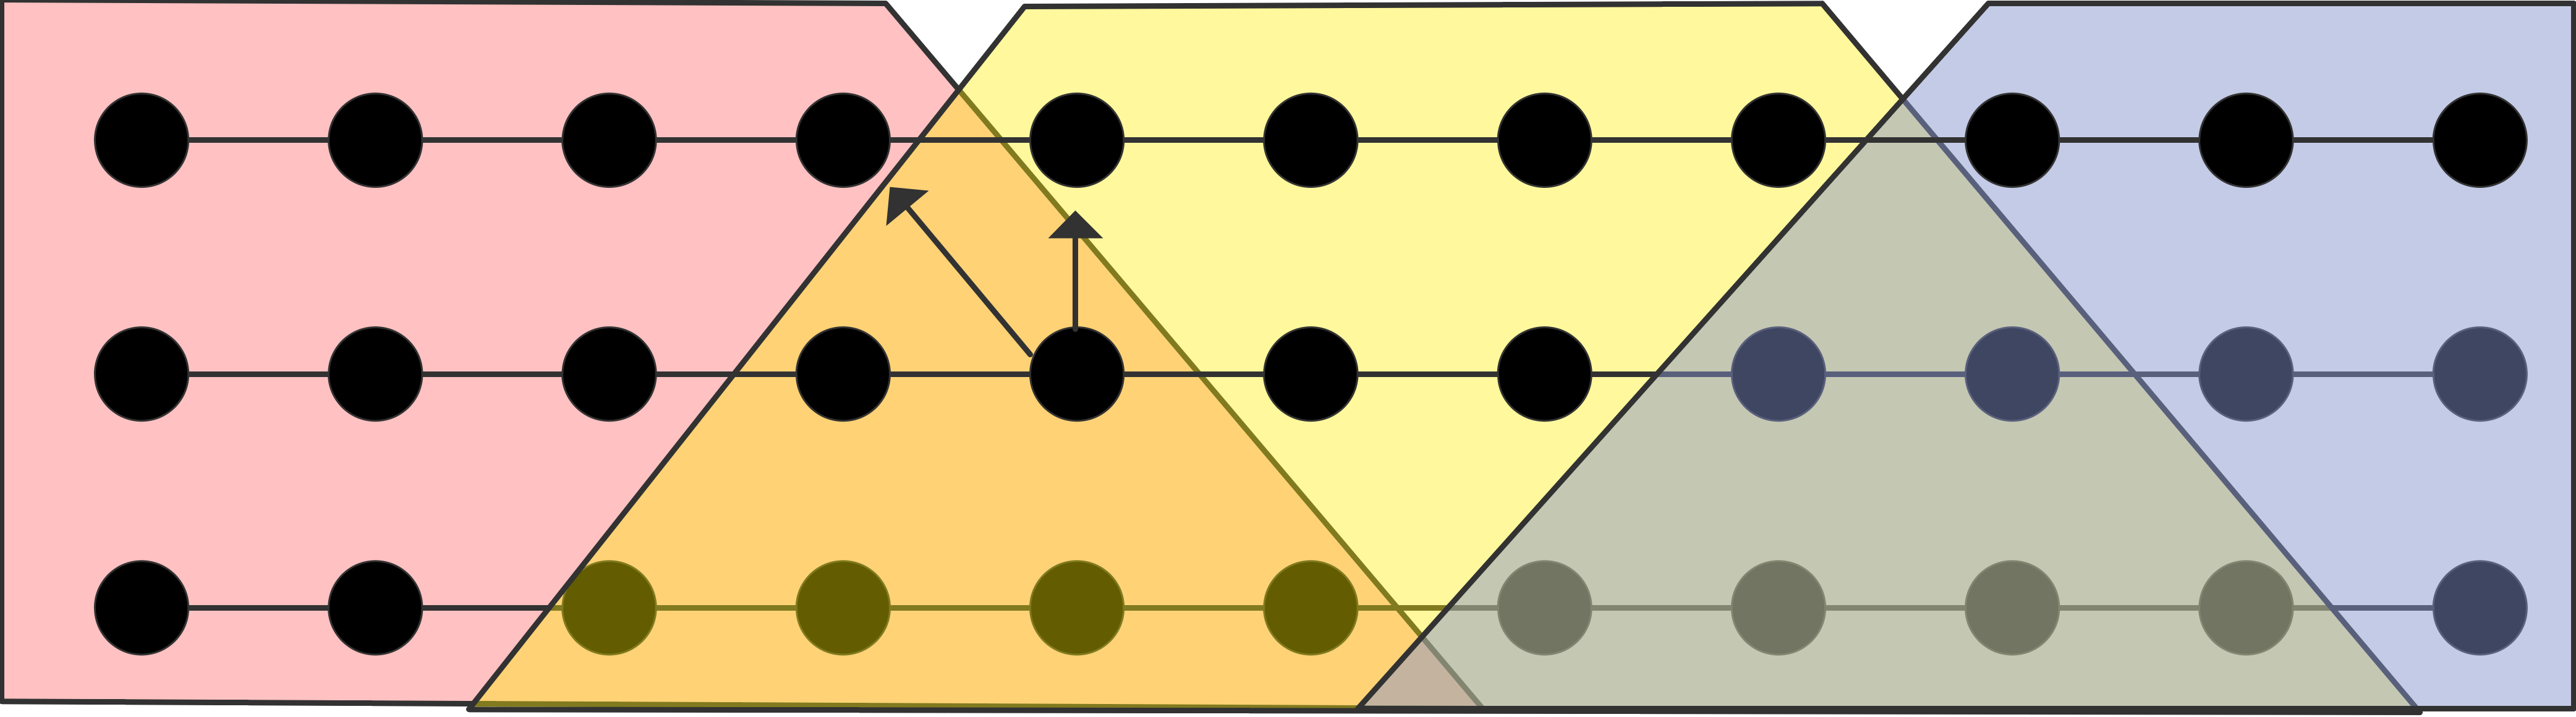
\includegraphics[scale=.1]{graphics/grid-update-overlap}
\caption{Computation of blocks of grid points over multiple iterations}
\label{fig:grid-update-overlap}
\end{figure}
The first processor computes 4~points on level $n+2$. For this it needs 5~points
from level $n+1$, and these need to be computed too, from 6~points on level~$n$.
We see that a processor apparently needs to collect a \indexterm{ghost region}
of width two, as opposed to just one for the regular single step update.
One of the points computed by the first processor is $x^{(n+2)}_3$,
which needs $x^{(n+1)}_4$. This point is also needed for the computation
of $x^{(n+2)}_4$, which belongs to the second processor.

The easiest solution is to let this sort of point on the intermediate
level \emph{redundantly computed}\index{redundant computation}, in 
the computation of both blocks where it is needed, on two different processors.

\begin{exercise}
  Can you think of cases where a point would be redundantly computed by
  more than two processors?
\end{exercise}

We can give several interpretations to this scheme of computing multiple
update steps by blocks. 
\begin{itemize}
\item First of all, as we motivated above, doing this 
on a single processor increases locality: if all points in a coloured block
(see the figure) fit in cache, we get reuse of the intermediate points.
\item Secondly, if we consider this as a scheme for distributed memory computation,
it reduces message traffic. Normally, for every update step the processors
need to exchange their boundary data. If we accept some redundant duplication
of work, we can now eliminate the data exchange for the intermediate levels.
The decrease in communication will typically outweigh the increase in work.
\end{itemize}

\begin{exercise}
  Discuss the case of using this strategy for multicore computation.
  What are the savings? What are the potential pitfalls?
\end{exercise}

\Level 1 {Analysis}

Let's analyze the algorithm we have just sketched.  As in
equation~\eqref{eq:3p-average} we limit ourselves to a 1D set of
points and a function of three points. The parameters describing the
problem are these:
\begin{itemize}
\item $N$ is the number of points to be updated, and $M$~denotes the
  number of update steps. Thus, we perform $MN$ function evaluations.
\item $\alpha,\beta,\gamma$ are the usual parameters describing
  latency, transmission time of a single point, and time for an
  operation (here taken to be an $f$ evaluation).
\item $b$ is the number of steps we block together.
\end{itemize}
Each halo communication consists of $b$ points, and we do this $\sqrt
N/b$ many times.  The work performed consists of the $MN/p$ local
updates, plus the redundant work because of the halo. The latter term
consists of $b^2/2$ operations, performed both on the left and right
side of the processor domain.

Adding all these terms together, we find a cost of
\[ \frac Mb\alpha+M\beta+\left(\frac {MN}p+Mb\right)\gamma. \]
We observe that the overhead of $\alpha M/b+\gamma Mb$ is independent of~$p$,
\begin{exercise}
  Compute the optimal value of~$b$, and remark that it only depends on
  the architectural parameters $\alpha,\beta,\gamma$ but not on the
  problem parameters.
\end{exercise}

\Level 1 {Communication and work minimizing strategy}

We can make this algorithm more efficient by 
\indextermsub{overlapping computation with}{communication}.
As illustrated in
figure~\ref{fig:grid-update-local}, each processor start by
communicating its halo, and overlapping this communication with the
part of the communication that can be done locally. The values that
depend on the halo will then be computed last.

\begin{figure}[ht]
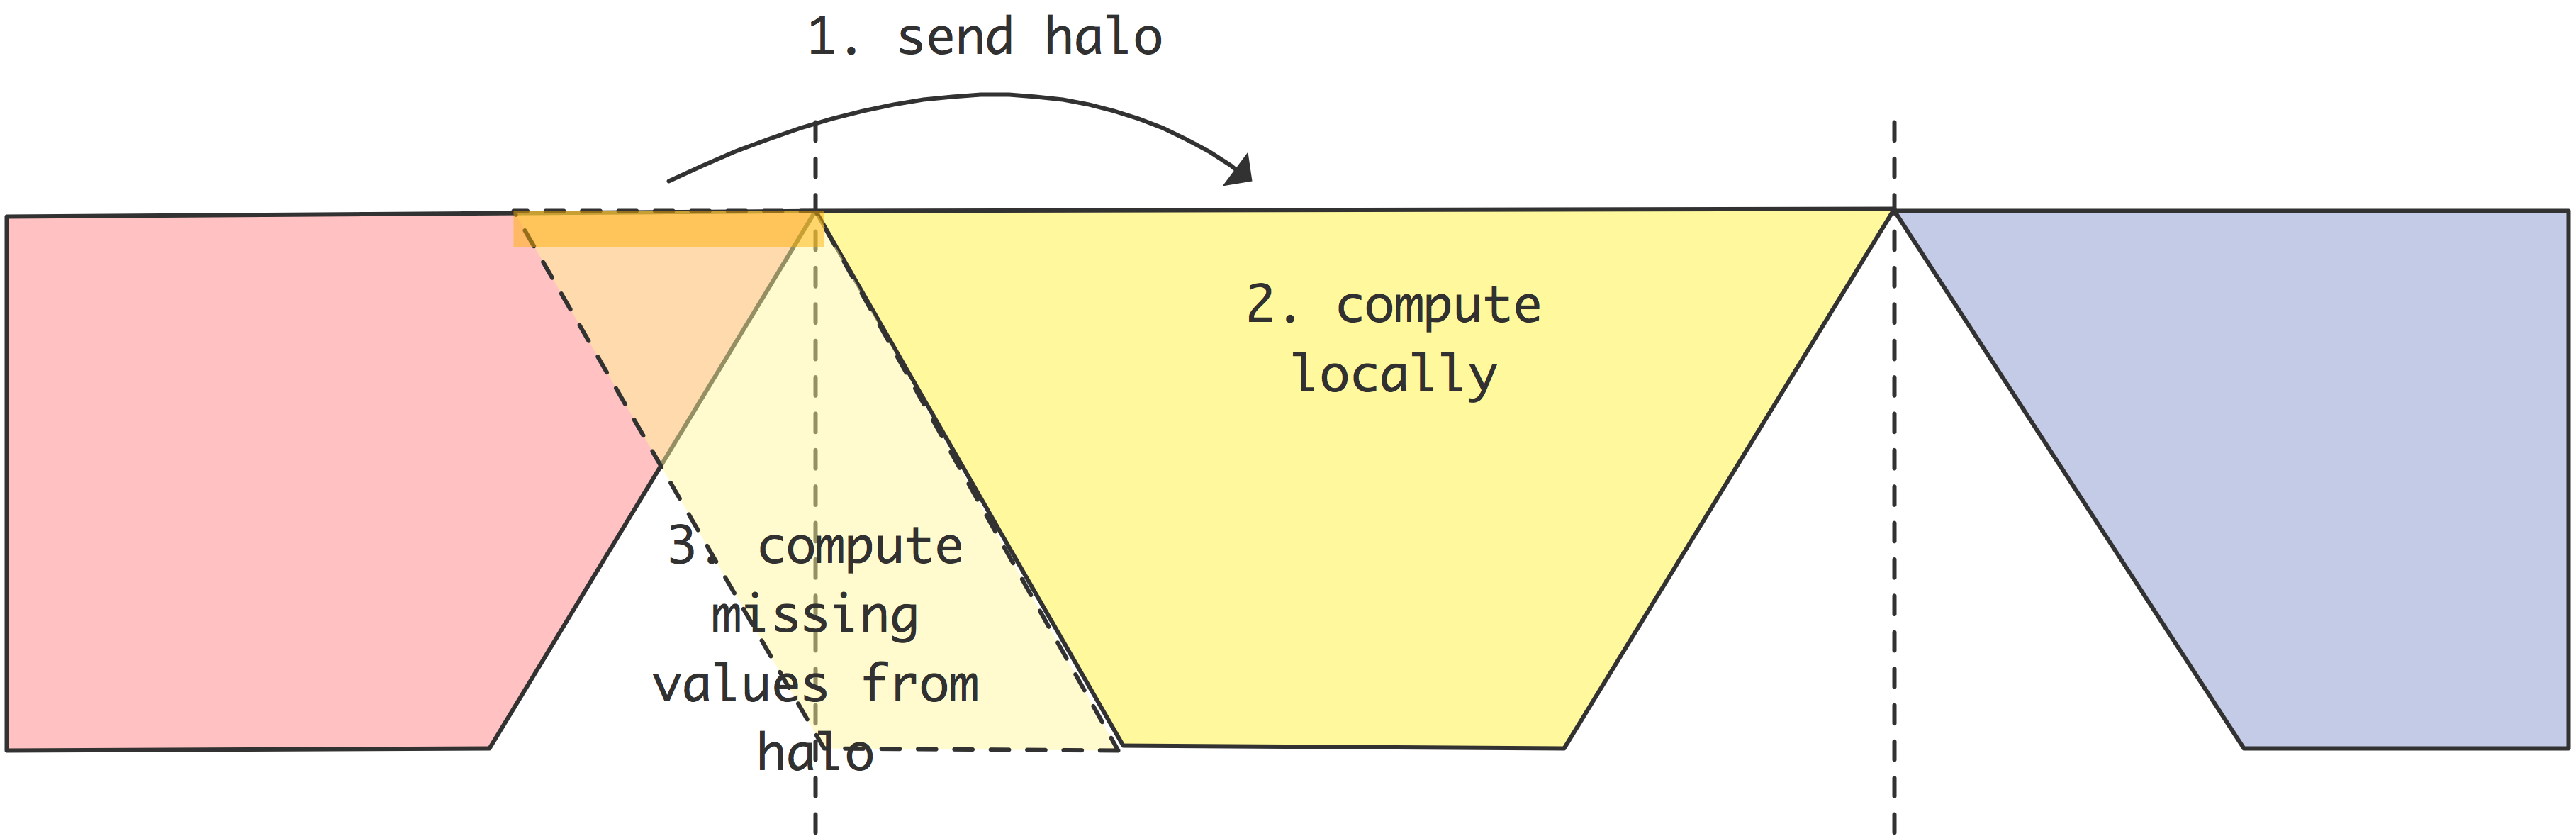
\includegraphics[scale=.1]{graphics/grid-update-local}
\caption{Computation of blocks of grid points over multiple iterations}
\label{fig:grid-update-local}
\end{figure}

\begin{exercise}
  What is a great practical problem with organizing your code (with
  the emphasis on `code'!) this way?
\end{exercise}

If the number of points per processor is large enough, the amount of
communication is low relative to the computation, and you could take
$b$ fairly large. However, these grid updates are mostly used in
iterative methods such as the \indexac{CG} method
(section~\ref{sec:cg}), and in that case considerations of roundoff
prevent you from taking $b$ too large\cite{ChGe:sstep}.

\begin{exercise}
  Go through the complexity analysis for the non-overlapping algorithm
  in case the points are organized in a 2D grid. Assume that each
  point update involves four neighbours, two in each coordinate
  direction.
\end{exercise}

A further refinement of the above algorithm is possible.
Figure~\ref{fig:grid-update-minimal} illustrates that it is possible
to use a halo region that uses different points from different time steps.
\begin{figure}[ht]
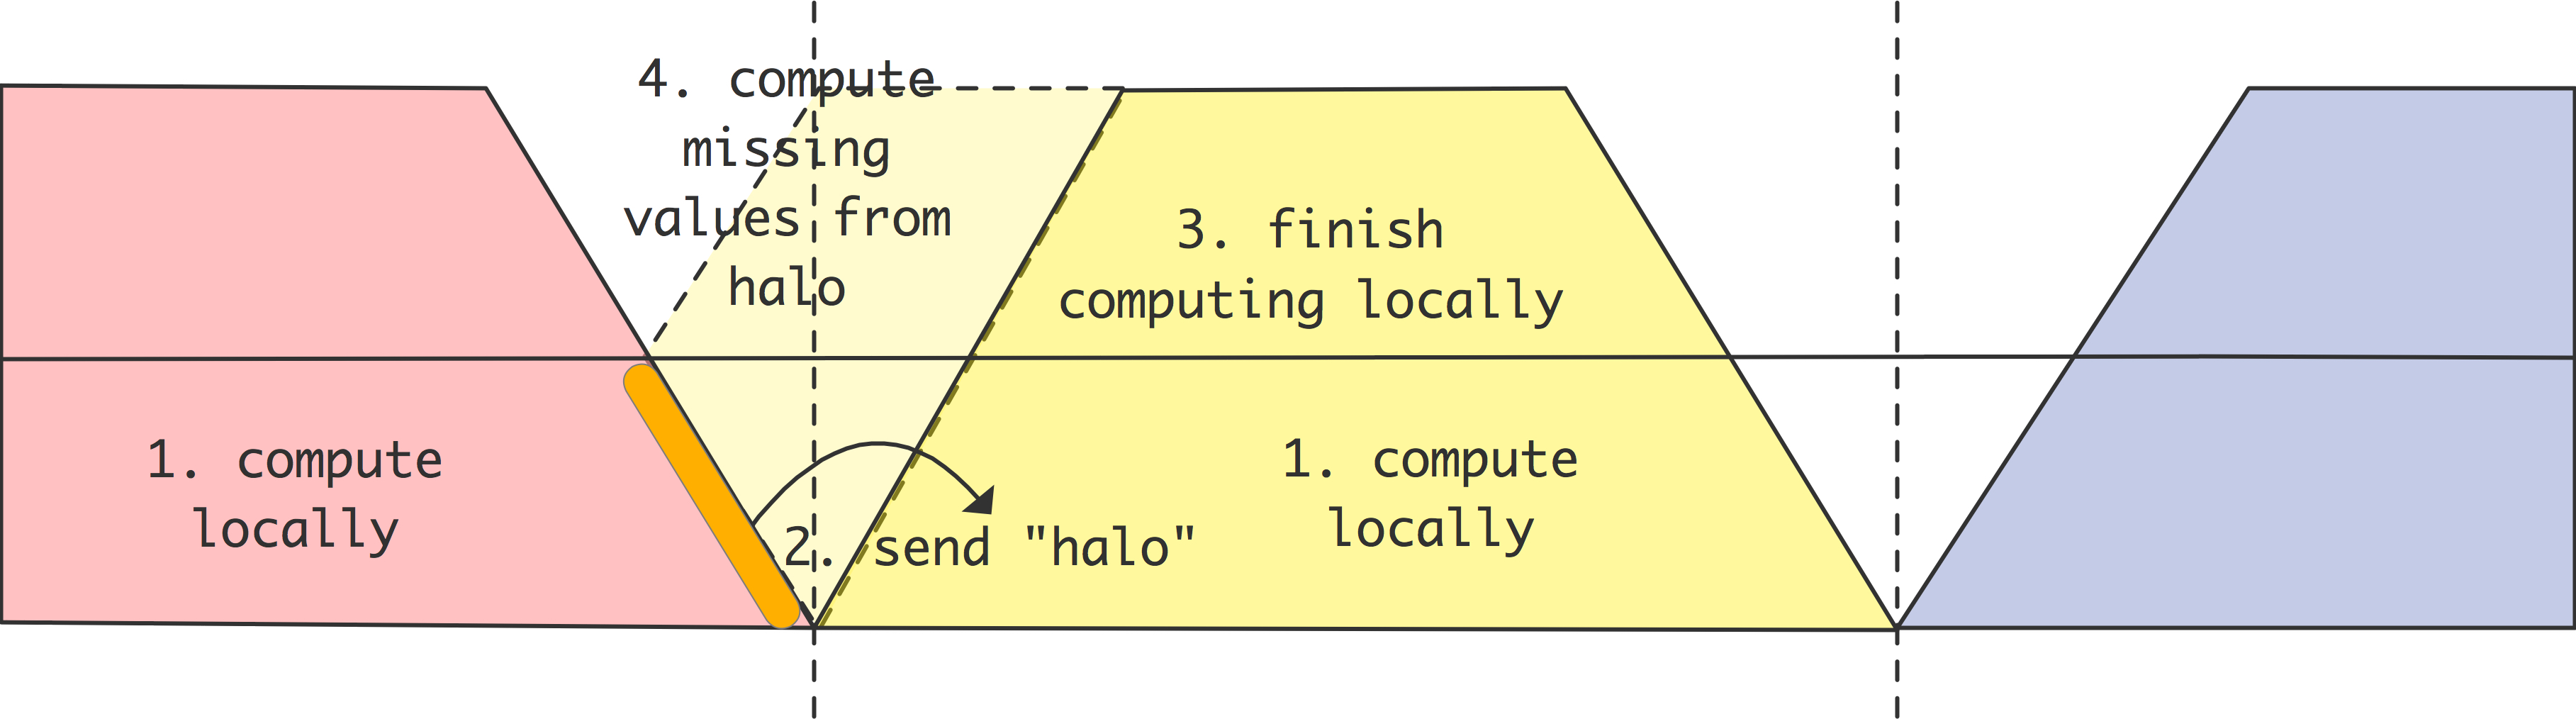
\includegraphics[scale=.1]{graphics/grid-update-minimal}
\caption{Computation of blocks of grid points over multiple iterations}
\label{fig:grid-update-minimal}
\end{figure}
This algorithm (see~\cite{Demmel2008IEEE:avoiding}) cuts down on the amount
of redundant computation. However, now the halo values that are communicated
first need to be computed, so this requires splitting the local communication
into two phases.

\Level 0 {Block algorithms on multicore architectures}
\label{sec:multicore-block}
\input chapters/ernie

